
The fragmentation of a $b$- or $c$-quark into a heavy flavor hadron is modeled by the
generators using a non-perturbative fragmentation function $D_{Q}^{H}(z,\mu^2)$ that describes
the probability that a quark of species $Q$ will fragment into a hadron of species $H$ carrying
fraction $z$ of the quark's momentum~\cite{PhysRevD.86.010001}.  As with parton distribution functions, the fragmentation
functions exhibit scaling violations and therefore must be evaluated at an appropriate
scale $\mu$.  These fragmentation functions are assumed to be universal, aside from the
scale dependence, which can be calculated perturbatively. Modeling of the fragmentation functions differs among the generators, but
in all cases the parameters of the models have been tuned using data from
$e^+e^-$ collisions.  

To assess the performance of the four generators, the following strategy is used.  First,
$e^+e^-\rightarrow b\overline b$  and $e^+e^-\rightarrow c\overline c$ samples are generated 
at the center-of-mass energy of the most accurate experimental measurements, using shower parametrizations consistent with those used for the LHC tunes.
%, which have hadronization parameters tuned using both LHC and LEP data.  
These samples
are used to validate the modeling of the non-perturbative heavy flavor fragmentation functions.
Second, the evolution of fragmentation functions is studied by comparing these samples with
$e^+e^-\rightarrow b\overline b$  and $e^+e^-\rightarrow c\overline c$ events generated at
$\sqrt{s}=200$~\GeV.  Third, the fragmentation is studied for each of the
generators in the process $pp \rightarrow t \overline t$, in which the production of $b$- and $c$-jets are predominantly produced from the \ttbar\ hard scatter. Finally, to study
the case where heavy flavor is produced both in the hard scatter and in the parton
shower, samples of high \pT\ jets are analyzed.

Data on $b$-quark
fragmentation are available from LEP and SLC.  The measurements 
parametrize the fragmentation function as a function of $x \equiv E/E_{\textrm\;beam}$ where
$E$ is the energy of the bottom hadron.  Figure~\ref{fig:lepfrag}~(a) compares the distribution 

$$F(x) \equiv \frac{1}{N_{B}} \frac{dN_{B}}{dx}$$

\noindent
for the four generators to measurements from DELPHI~\cite{DELPHI}  and SLD~\cite{SLD}~. The mean values of these distributions are given in Table~\ref{t:lepfrag}.
To better match the experimental requirements on these measurements, events in the MC samples
are required to satisfy the criteria that $|\cos{\theta}_{\textrm\;thrust}|<$ 0.7 ~\footnote{The thrust axis is defined as the axis {\textbf n} that maximizes the value of${\sum\limits_{i} {\textbf n} \cdot {\textbf p_i}}/{\sum\limits_{i} {\textbf p_i} }$, where the sum is taken over all stable particles in the event.} and that
the number of weakly decaying bottom hadrons ($N_B$) satisfy $0 < N_{B}  < 3$.  The mean value of $x$
in the MC samples varies from $0.6782\pm 0.0005$ (\Herwig) to $0.7303\pm 0.0005$ (\PythiaE).
\Pythia\ and \Herwigpp\ agree well with the data, while \PythiaE\ is high by $\sim 2\%$ and
\Herwig\ is low by $\sim 3\%$.  These results are consistent with those presented in Reference~\cite{Karneyeu:2013aha}.

Figure~\ref{fig:lepfrag}~(b) shows the same distribution
for the four generators at a center-of-mass energy of $\sqrt{s}=200$~GeV.  The samples are generated without initial state QED in order to isolate the effect of increased $\sqrt{s}$.  As expected,
the mean value of $x$ is lower than at the $Z$-pole, due the evolution of the
fragmentation function.  The ratio of the means at the higher energy to those at the 
lower energy are 93.8\%, 95.8\%, 94.0\%\ and 97.2\% for \PythiaE, \Pythia, \Herwigpp\ and \Herwig\ 
respectively.

Studies of $c$-quark fragmentation are available from Belle~\cite{Belle} and CLEO~\cite{CLEO}. 
The fragmentation function is measured as a function of $x_p \equiv p/p_{\textrm\;max}$ where
$p$ is the momentum of the charm hadron and $p_{\textrm\;max}$ is the maximum momentum that
is kinematically allowed.  Charm hadrons are required to be directly produced; bottom hadron decay products are
excluded.
Figures~\ref{fig:belle}~(a) and ~\ref{fig:belle}~(b) compare the four generators to the experimental measurements for $D^+$ and
$D^0$ mesons respectively. Table~\ref{t:belle}~ gives the mean value of the fragmentation functions. The \PythiaE\ fragmentation appears to be significantly harder than the data, while 
other generators agree reasonably well with the data and with each other.
%n hadron collisions...sentence changed. I THINK physics is right...

In $e^+e^-$ collisions, the fragmentation function can be measured relative to the beam energy, since the 
momentum transfer of the hard scatter is fixed by the energy of the initial beams (aside from initial state photon radiation). However, fragmentation in hadron collisions must be parameterized with respect to the output of a jet-finding algorithm. By convention, the \pT\ of the jet containing the
heavy flavor hadron is used to approximate the unknown \pT\ of the heavy flavor parton.
The resulting fragmentation function $f(z)$ is defined to be

$$
f(z) \equiv \frac{\vec{p}_{\textrm\;hadron} \cdot \vec{p}_{\textrm\;jet} } {{p^2}_{\textrm\;jet}}.
$$
\noindent

For this study, the $f(z)$ is measured for \antiktfour\ jets with $|\eta^{\textrm\;jet}| < 2.5$.  Jets are defined
to be heavy flavor jets if there is a weakly decaying heavy flavor hadron with $\pt>5$\,\GeV\ 
%with transverse momentum $\pt>25$\,\GeV\ 
%containing a weakly decaying heavy flavor hadron with $\pt>5$\,\GeV\ 
within $\Delta R=\sqrt{\Delta \phi^2 +\Delta \eta^2}<0.3$ of the jet direction.
For measurements of the charm fragmentation function, jets are vetoed if the charm
hadron contained in the jet is a bottom hadron decay product. 

 For large momentum scale processes,
an additional perturbative contribution (from $g\rightarrow b \overline b$) becomes significant. 
In some cases, this perturbative component is explicitly included in
the matrix element calculation, while in other cases this component is treated as part
of the parton shower. Such jets are included here in the definition of $b$- and $c$- jets.

Figure~\ref{fig:tfrag} and Table~\ref{t:tfrag} show the  bottom and  charm fragmentation functions $f(z)$ for  
jets in the \ttbar\ samples satisfying the requirement \ptJet\ \textgreater~25~\GeV\ 
in events containing a lepton with $p_T^{\textrm\;lep} > 20$ GeV and $|\eta^{\textrm\;lep}| < 2.5$. The mean value of $z$ varies from 0.741 (\Herwig) to 0.772 (\Herwigpp) for $b$-quarks
and from 0.552 (\Pythia) to 0.575 (\Herwig) for $c$-quarks.  The $b$-quark ($c$-quark) fragmentation in 
\Herwigpp\ (\Herwig) is noticeably harder than for the other generators.

The fragmentation function in jets is sensitive to many other aspects of the simulation. Measurements
depend on the choice of jet algorithm and can be affected by the underlying event tune, as well as by the
transverse shape of the generated jet.  Details of the shower modeling itself, such as the suppression of 
QCD radiation from heavy particles (the \textit{dead-cone} effect~\cite{Marchesini:1989yk}) can also play a role.
%Such effects can result in differences for the lighter charm and the heavier bottom.
To better study the fragmentation model, these effects are probed using additional distributions
for these heavy flavor jets.  Figure~\ref{fig:twidth} shows the width of the 
$b$-quark and  $c$-quark jets, where the jet width ($W$) is obtained from the \pT\ weighted
distribution of the distance $\Delta R$ from the center of the jet: 

$$
W \equiv \frac{\sum_{i} {p_{T}}_i \; \Delta R_{i}}{\sum_{i} {p_{T}}_i}
$$
\noindent
and the sum is taken over all stable particles that are constituents of the jets.    The mean value
of the jet widths for all generators agree to within a few percent, although the distribution of
widths for $b$-quark jets is slightly broader for \PythiaE\ than for the other generators and the
distribution of widths for $c$-quarks is slightly narrower for \Herwig\ and \Herwigpp\
than for \Pythia\ and \PythiaE.

\begin{figure}
\centering
\begin{subfigure}[]{0.45\textwidth}
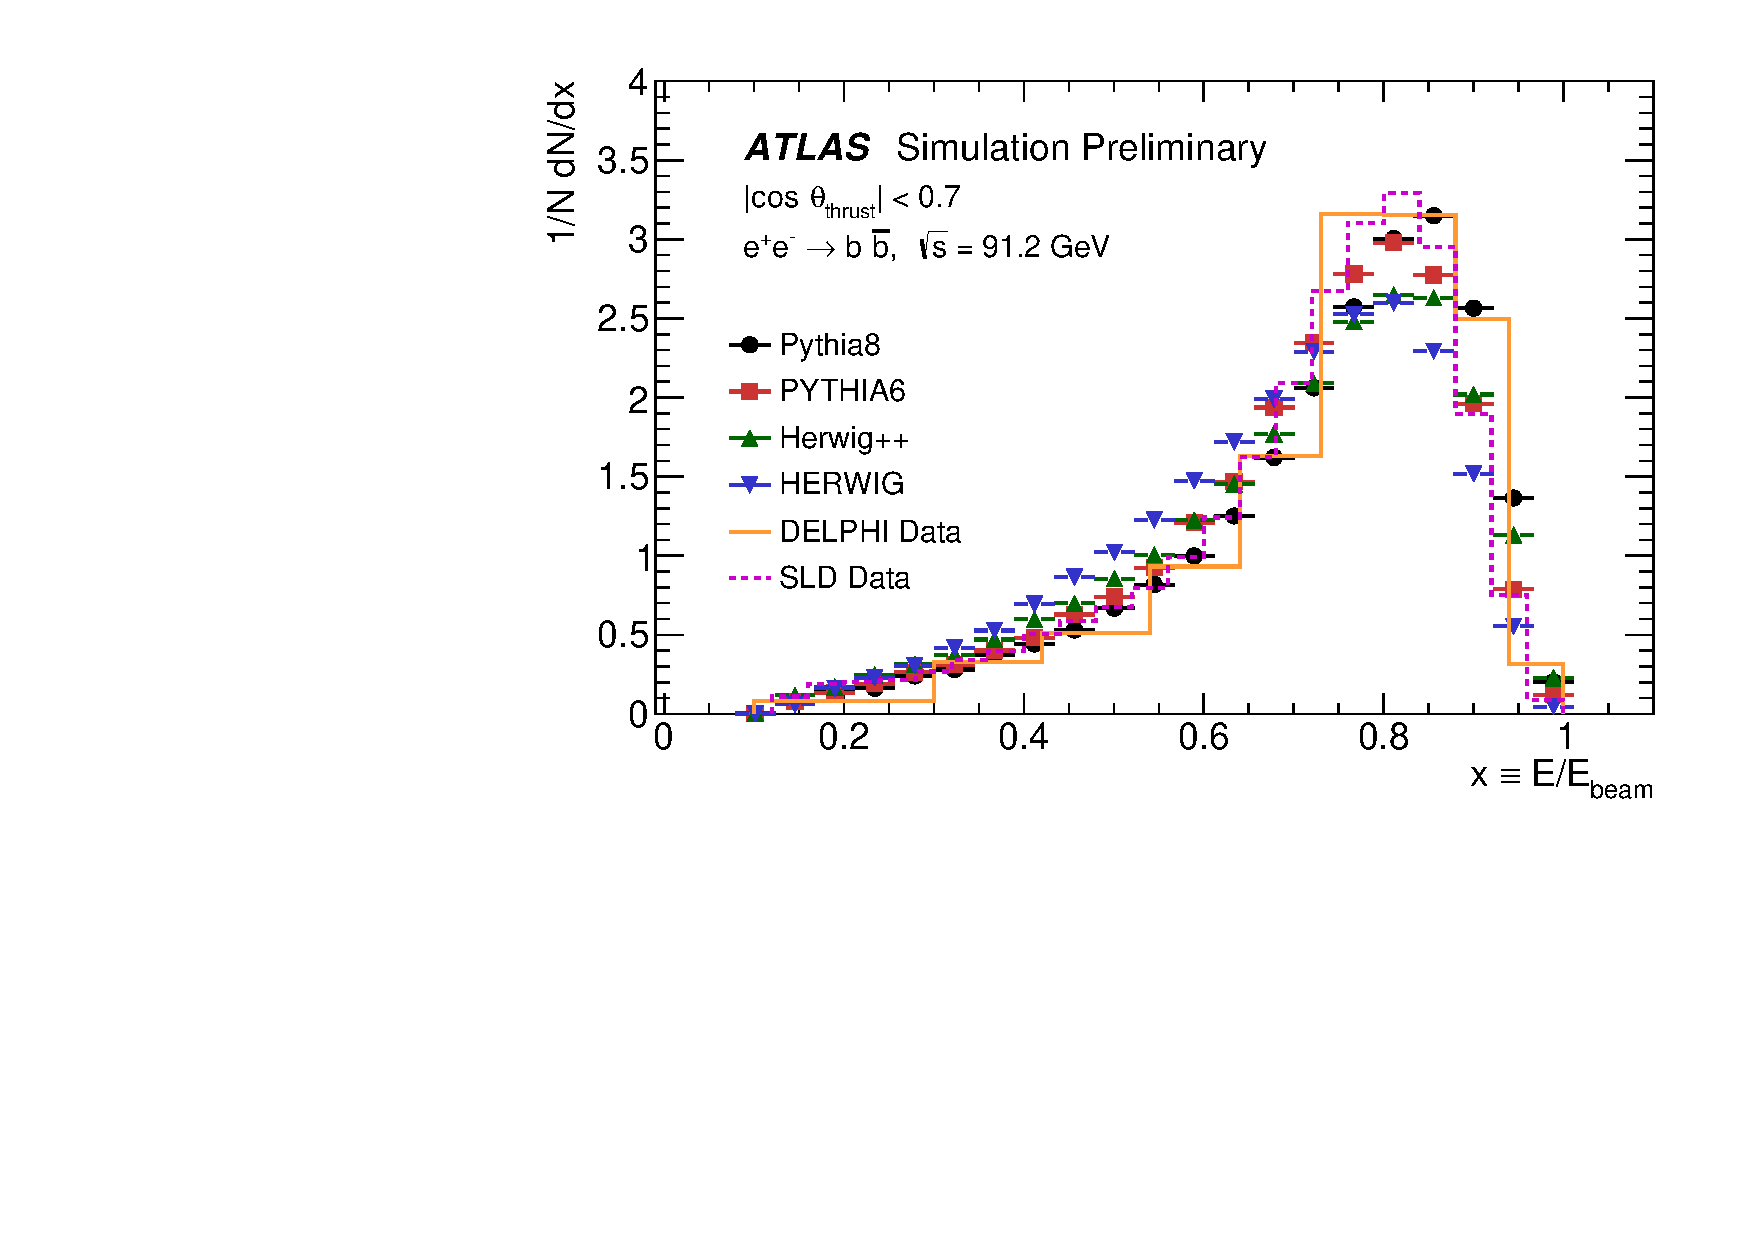
\includegraphics[width=\textwidth]{evtgen/figures/Frag/LEP.pdf}
\end{subfigure}
\begin{subfigure}[]{0.45\textwidth}
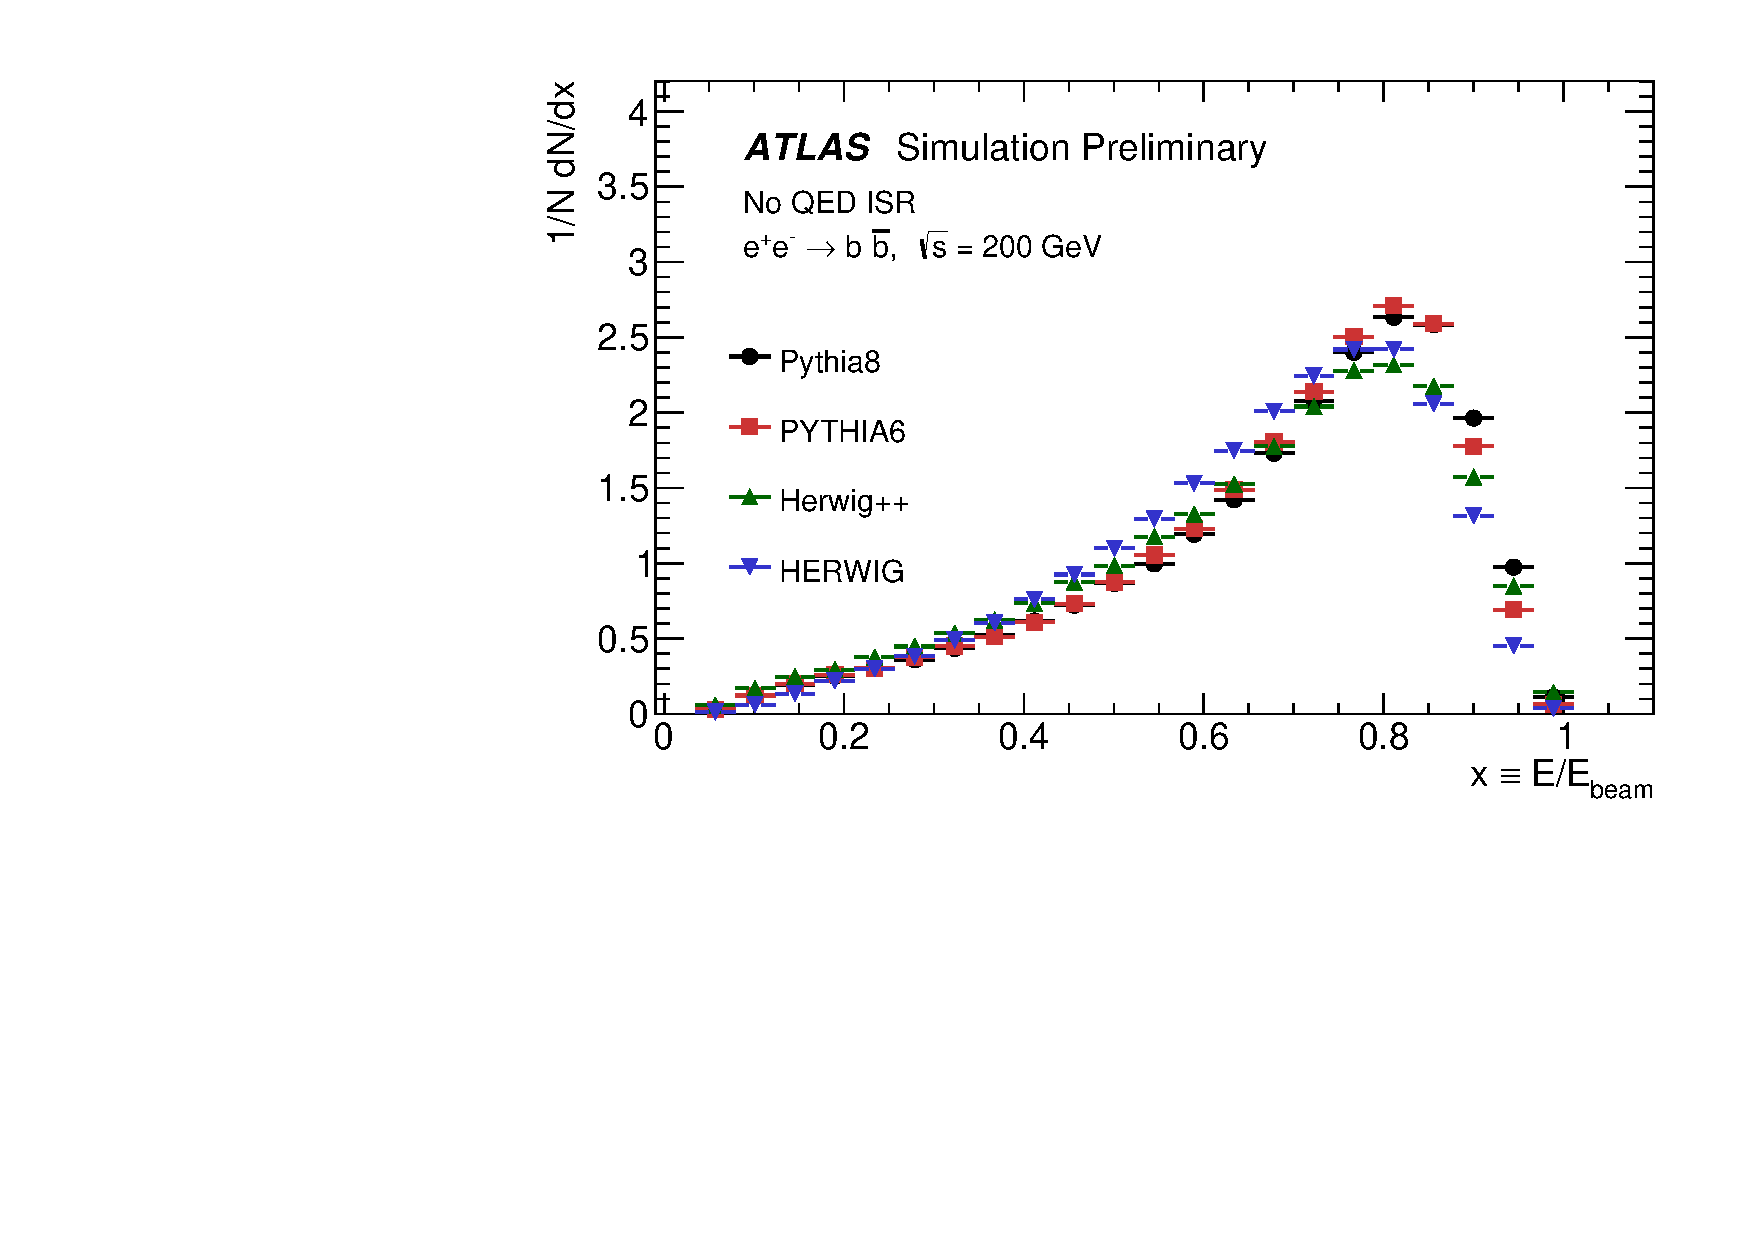
\includegraphics[width=\textwidth]{evtgen/figures/Frag/200GeV/h_Xweak_B.pdf}
\end{subfigure}
\caption{The $b$-quark fragmentation function obtained 
with \PythiaE, \Pythia, \Herwigpp\ and \Herwig\  
for (a)~$\sqrt{s}=91.2$~\GeV\ and (b)~$\sqrt{s}=200$~\GeV\ $e+e-$ collisions. 
DELPHI and SLD data in (a) are taken from References~\cite{DELPHI} and~\cite{SLD} respectively and are plotted without error bars.  }
\label{fig:lepfrag}
\end{figure}


\begin{table}
\begin{center}
\begin{tabular}{|r|r|}
\hline
\multicolumn{2}{|c|}{$E_{B}/E_{beam}$} \\
\hline
\hline
 \PythiaE & $0.7303 \pm 0.0005$ \\
 \Pythia & $0.7090 \pm 0.0005$ \\
 \Herwigpp & $0.7012 \pm 0.0006$ \\
 \Herwig  & $0.6782 \pm 0.0005$ \\
\hline
 Delphi Data & $0.699 \pm 0.011$ \\
 SLD Data & $0.709 \pm 0.005$ \\
\hline 

\hline
\end{tabular}
\caption{The mean $b$-quark fragmentation function obtained 
with \PythiaE, \Pythia, \Herwigpp\ and \Herwig\  
for $\sqrt{s}=91.2$~\GeV\ in $e+e-$ collisions. 
DELPHI and SLD data in (a) are taken from References~\cite{DELPHI} and~\cite{SLD} respectively.}
\label{t:lepfrag}
\end{center}%
\end{table}

\begin{figure}
\centering
 \begin{subfigure}[]{0.45\textwidth}
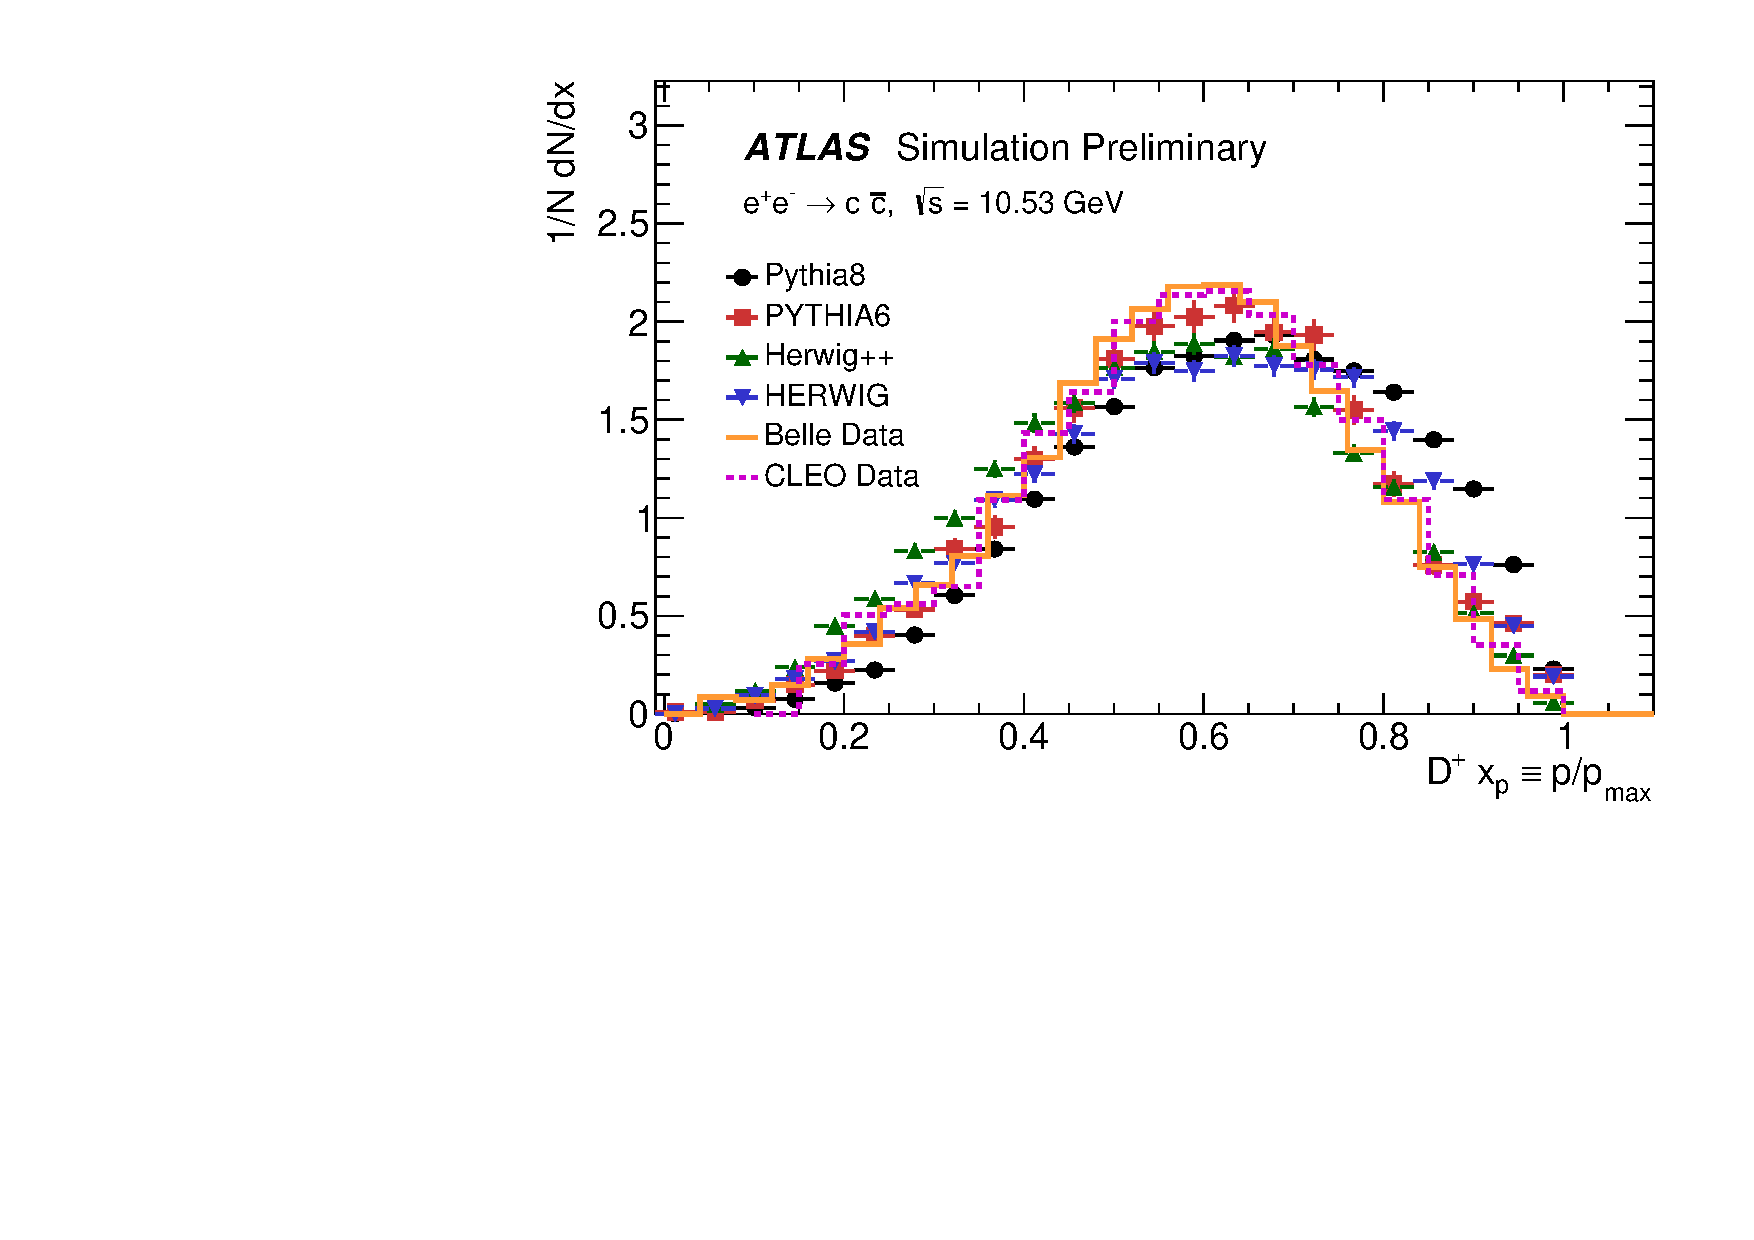
\includegraphics[width=\textwidth]{evtgen/figures/Frag/DPlusFrag.pdf}
\end{subfigure}
 \begin{subfigure}[]{0.45\textwidth}
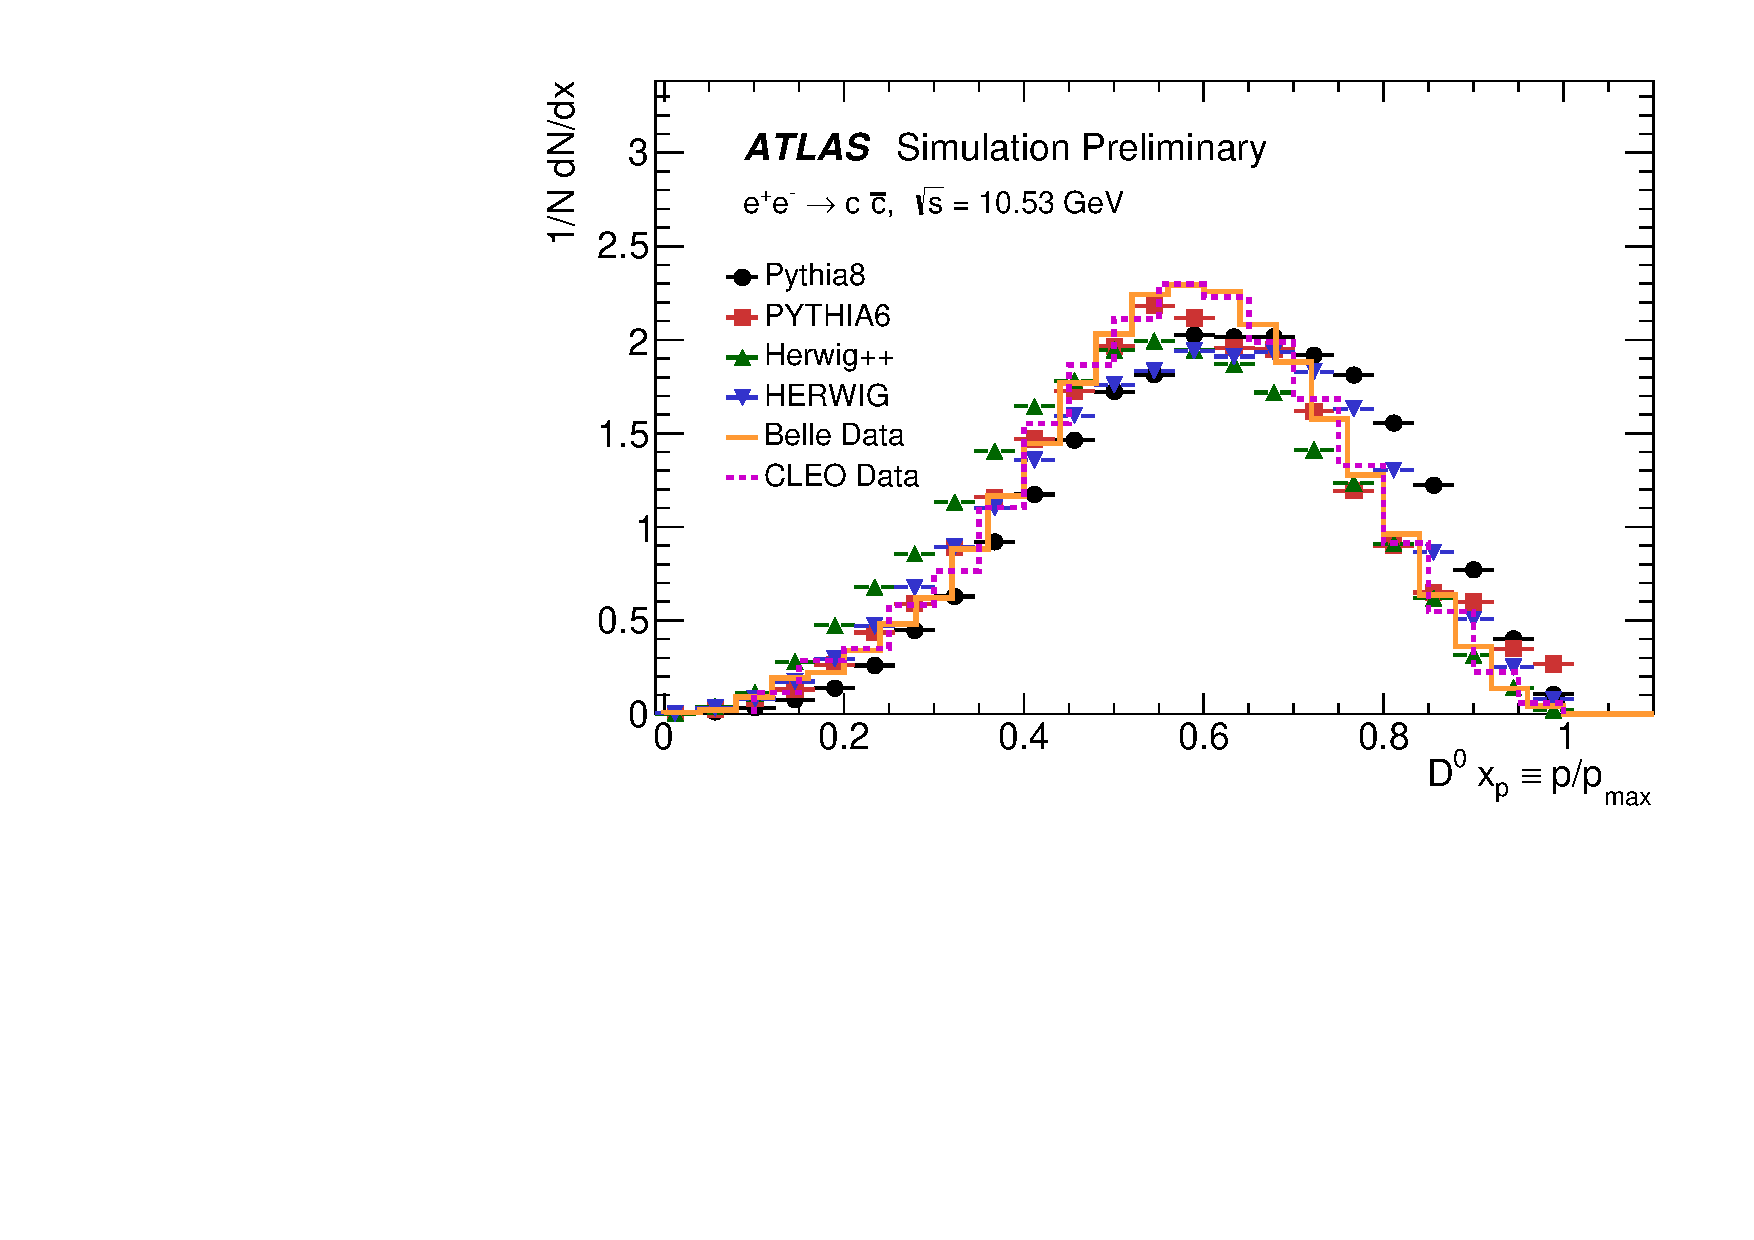
\includegraphics[width=\textwidth]{evtgen/figures/Frag/D0Frag.pdf}
\end{subfigure}
\begin{subfigure}[]{0.45\textwidth}
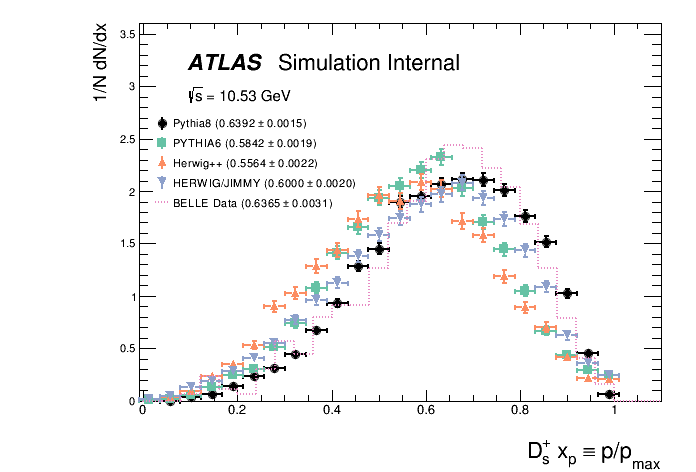
\includegraphics[width=\textwidth]{evtgen/figures/Frag/DSplusFrag.pdf}
\end{subfigure}
\caption{The $c$-quark fragmentation function obtained 
with \PythiaE, \Pythia, \Herwigpp\ and \Herwig\  
for $\sqrt{s}=10.53$~\GeV\ for $e+e-$ collisions for
(a)~$D^+$ and (b)~$D^0$ mesons. CLEO and Belle data are taken from References~\cite{CLEO} and~\cite{Belle}
respectively and are plotted without error bars. }
\label{fig:belle}
\end{figure}

\begin{table}
\begin{center}
\begin{tabular}{|r|r|r|}
\hline
\multicolumn{3}{|c|}{$p_{C}/p_{max}$} \\
\hline
& $D^+$ & $D^0$ \\
\hline
\hline
 \PythiaE & $0.6337 \pm 0.0010$ & $0.6156 \pm 0.0007$ \\
 \Pythia & $0.5918 \pm 0.0022$ & $0.5744 \pm 0.0011$ \\
 \Herwigpp & $0.5611 \pm 0.0016$ & $0.5390 \pm 0.0010$ \\
 \Herwig  & $0.5981 \pm 0.0016$ & $0.5797 \pm 0.0011$ \\
\hline
 Belle Data & $0.578 \pm 0.00148$ & $0.5703 \pm 0.0020$ \\
CLEO Data & $0.582 \pm 0.009$ & $0.570 \pm 0.006$ \\
\hline 

\hline
\end{tabular}
\caption{The mean $c$-quark fragmentation function obtained 
with \PythiaE, \Pythia, \Herwigpp\ and \Herwig\  
for $\sqrt{s}=10.53$~\GeV\ for $e+e-$ collisions for
(a)~$D^+$ and (b)~$D^0$ mesons. CLEO and Belle data are taken from References~\cite{CLEO} and~\cite{Belle}
respectively.}
\label{t:belle}
\end{center}%
\end{table}


\begin{figure}
\centering
\begin{subfigure}[]{0.45\textwidth}
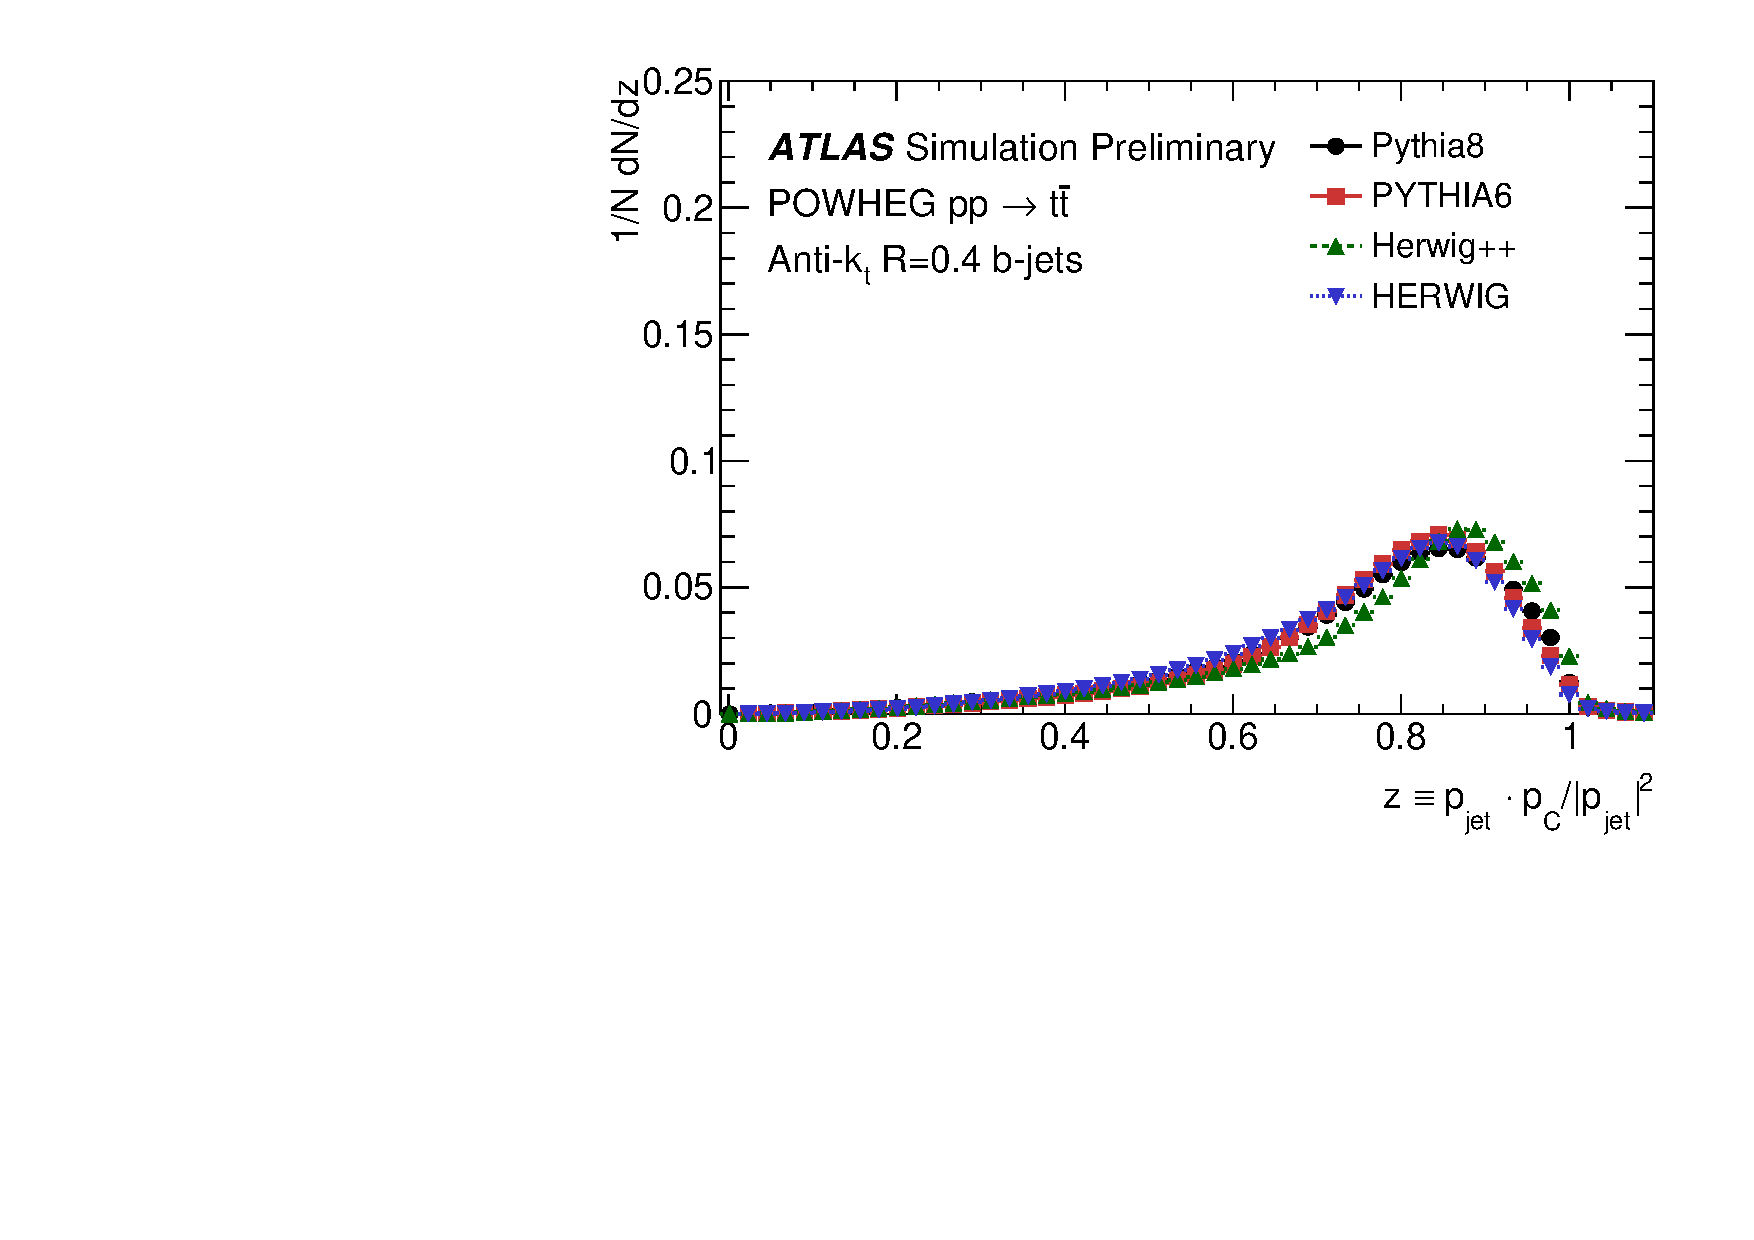
\includegraphics[width=\textwidth]{evtgen/figures/Frag/Top/h_BFrag_SingleHad.pdf}
\end{subfigure}
\begin{subfigure}[]{0.45\textwidth}
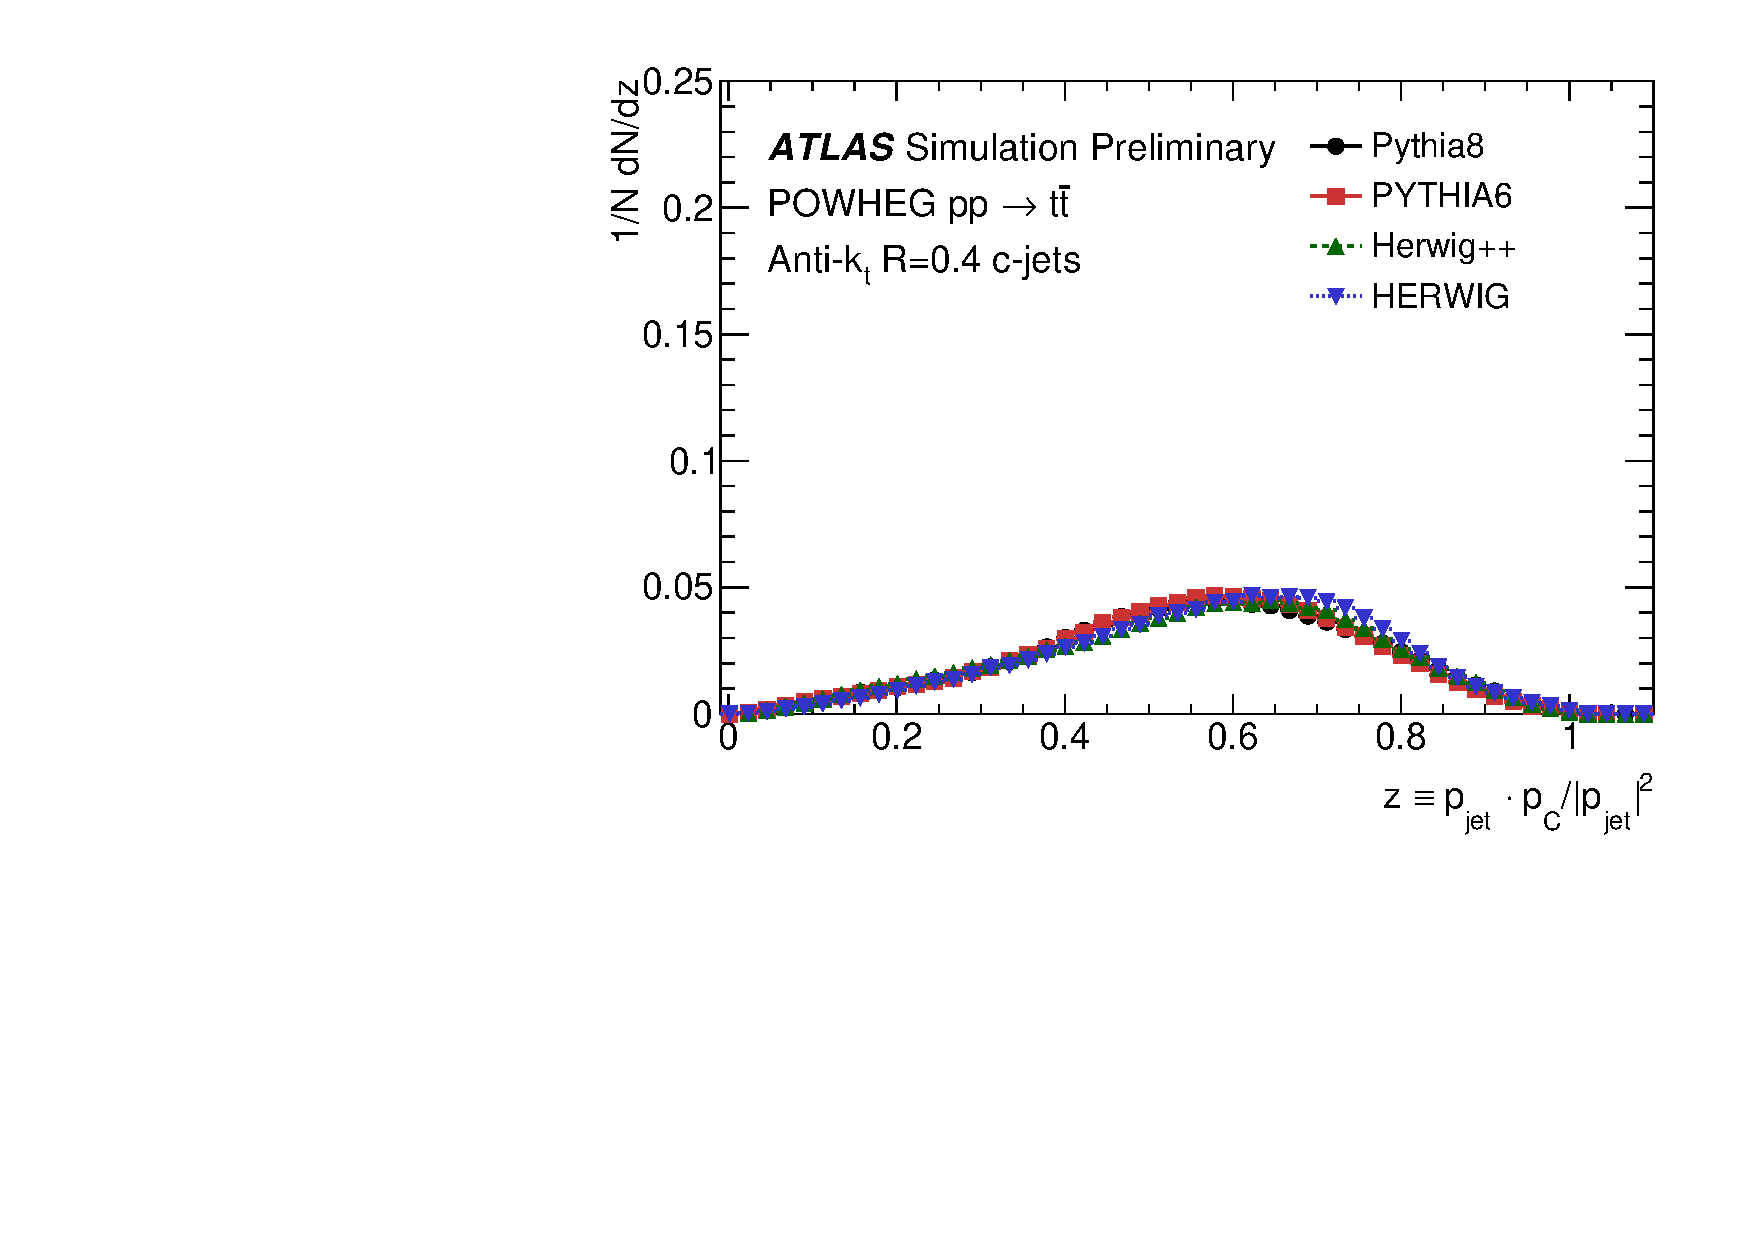
\includegraphics[width=\textwidth]{evtgen/figures/Frag/Top/h_CFrag_SingleHad.pdf}
\end{subfigure}
\caption{The fragmentation function for 
%(a)~$b$-jets and (b)~$c$-jets in \PowHeg\
%\ttbar\ samples where  \PythiaE, \Pythia, \Herwigpp\ and \Herwig\ have been used 
for the parton shower, hadronization and underlying event modeling.}
\label{fig:tfrag}
\end{figure}

\begin{table}
\begin{center}
\begin{tabular}{|r|r|r|}
\hline
Generator & $p_{jet} \cdot p_{B}/p_{jet}^2$  & $p_{jet} \cdot p_{C}/p_{jet}^2$ \\
\hline
 \PythiaE & $0.7529 \pm 0.0001$ & $0.5550 \pm 0.0004$  \\
 \Pythia & $0.7561 \pm 0.0001$  & $0.5525 \pm 0.0004$  \\
 \Herwigpp & $0.7719 \pm 0.0001$   & $0.5590 \pm 0.0004$  \\
 \Herwig  & $0.7411 \pm 0.0001$  & $0.5751 \pm 0.0004$  \\

\hline
\end{tabular}
\caption{The mean fragmentation function for 
$b$-jets and  $c$-jets in \PowHeg\
\ttbar\ samples where  \PythiaE, \Pythia, \Herwigpp\ and \Herwig\ have been used 
for the parton shower, hadronization and underlying event modeling.}
\label{t:tfrag}
\end{center}%
\end{table}

\begin{figure}
\centering
\begin{subfigure}[]{0.45\textwidth}
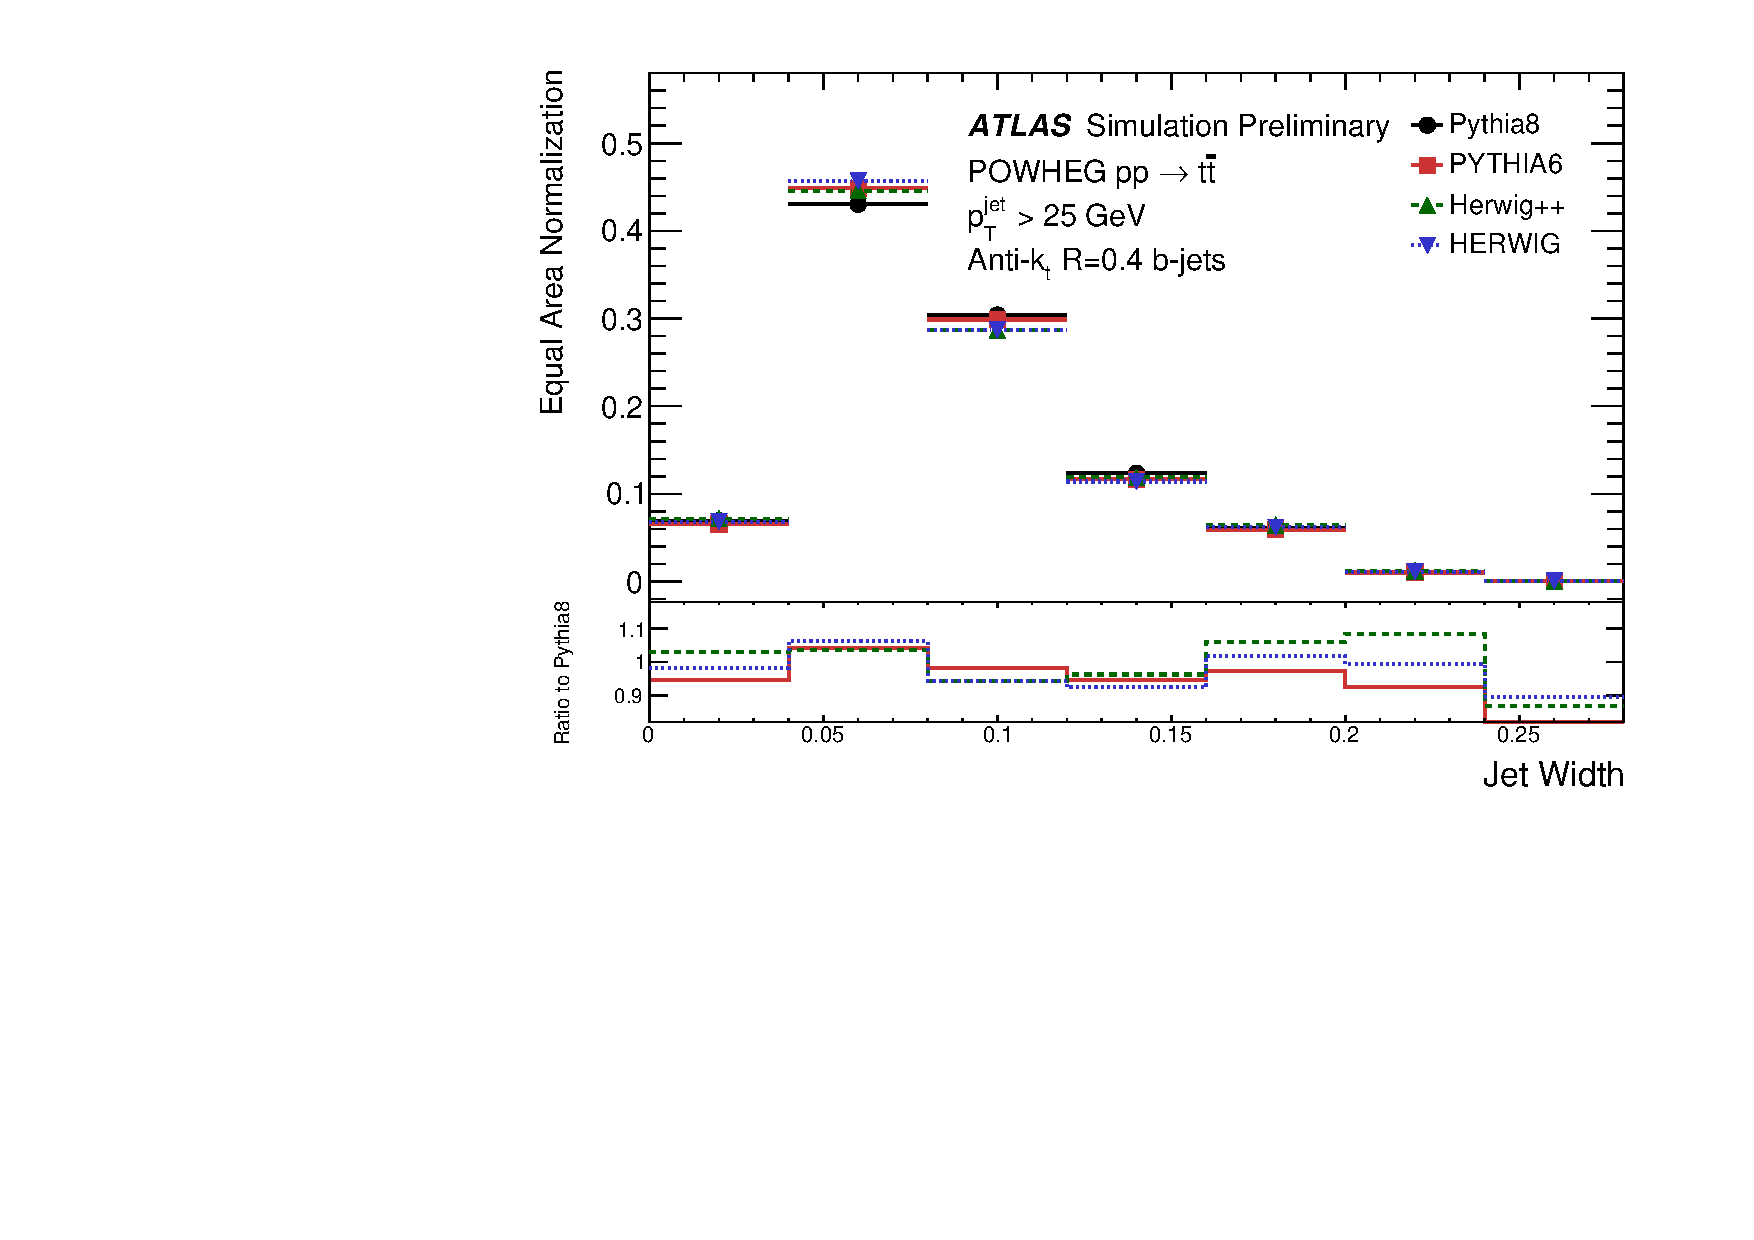
\includegraphics[width=\textwidth]{evtgen/figures/Frag/Top/SingleB/h_JetWidth.pdf}
\end{subfigure}
\begin{subfigure}[]{0.45\textwidth}
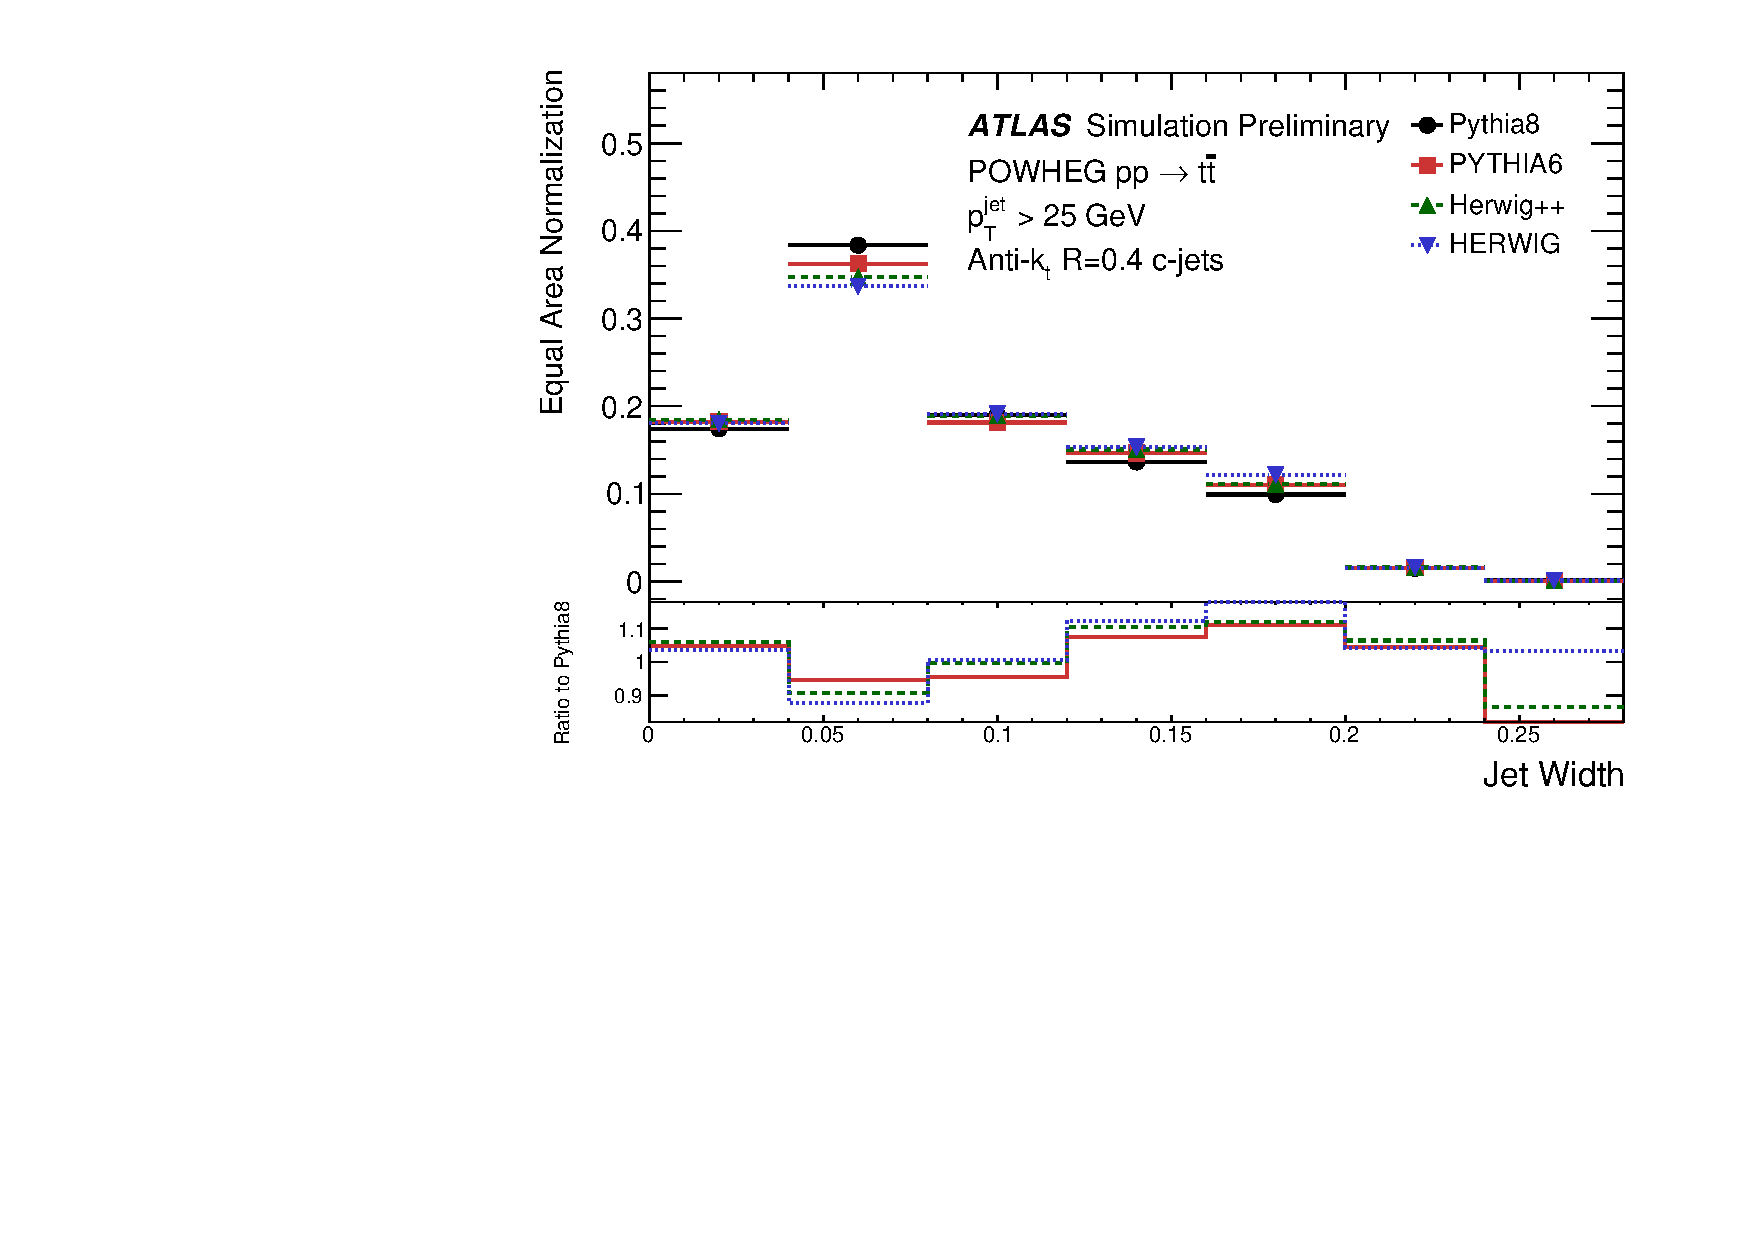
\includegraphics[width=\textwidth]{evtgen/figures/Frag/Top/SingleC/h_JetWidth.pdf}
\end{subfigure}
\caption{The jet width for 
(a)~$b$-jets and (b)~$c$-jets in \PowHeg\
\ttbar\ samples where  \PythiaE, \Pythia, \Herwigpp\ and \Herwig\ have been used 
for the parton shower, hadronization and underlying event modeling. }
\label{fig:twidth}
\end{figure}

\begin{figure}
\centering
\begin{subfigure}[]{0.45\textwidth}
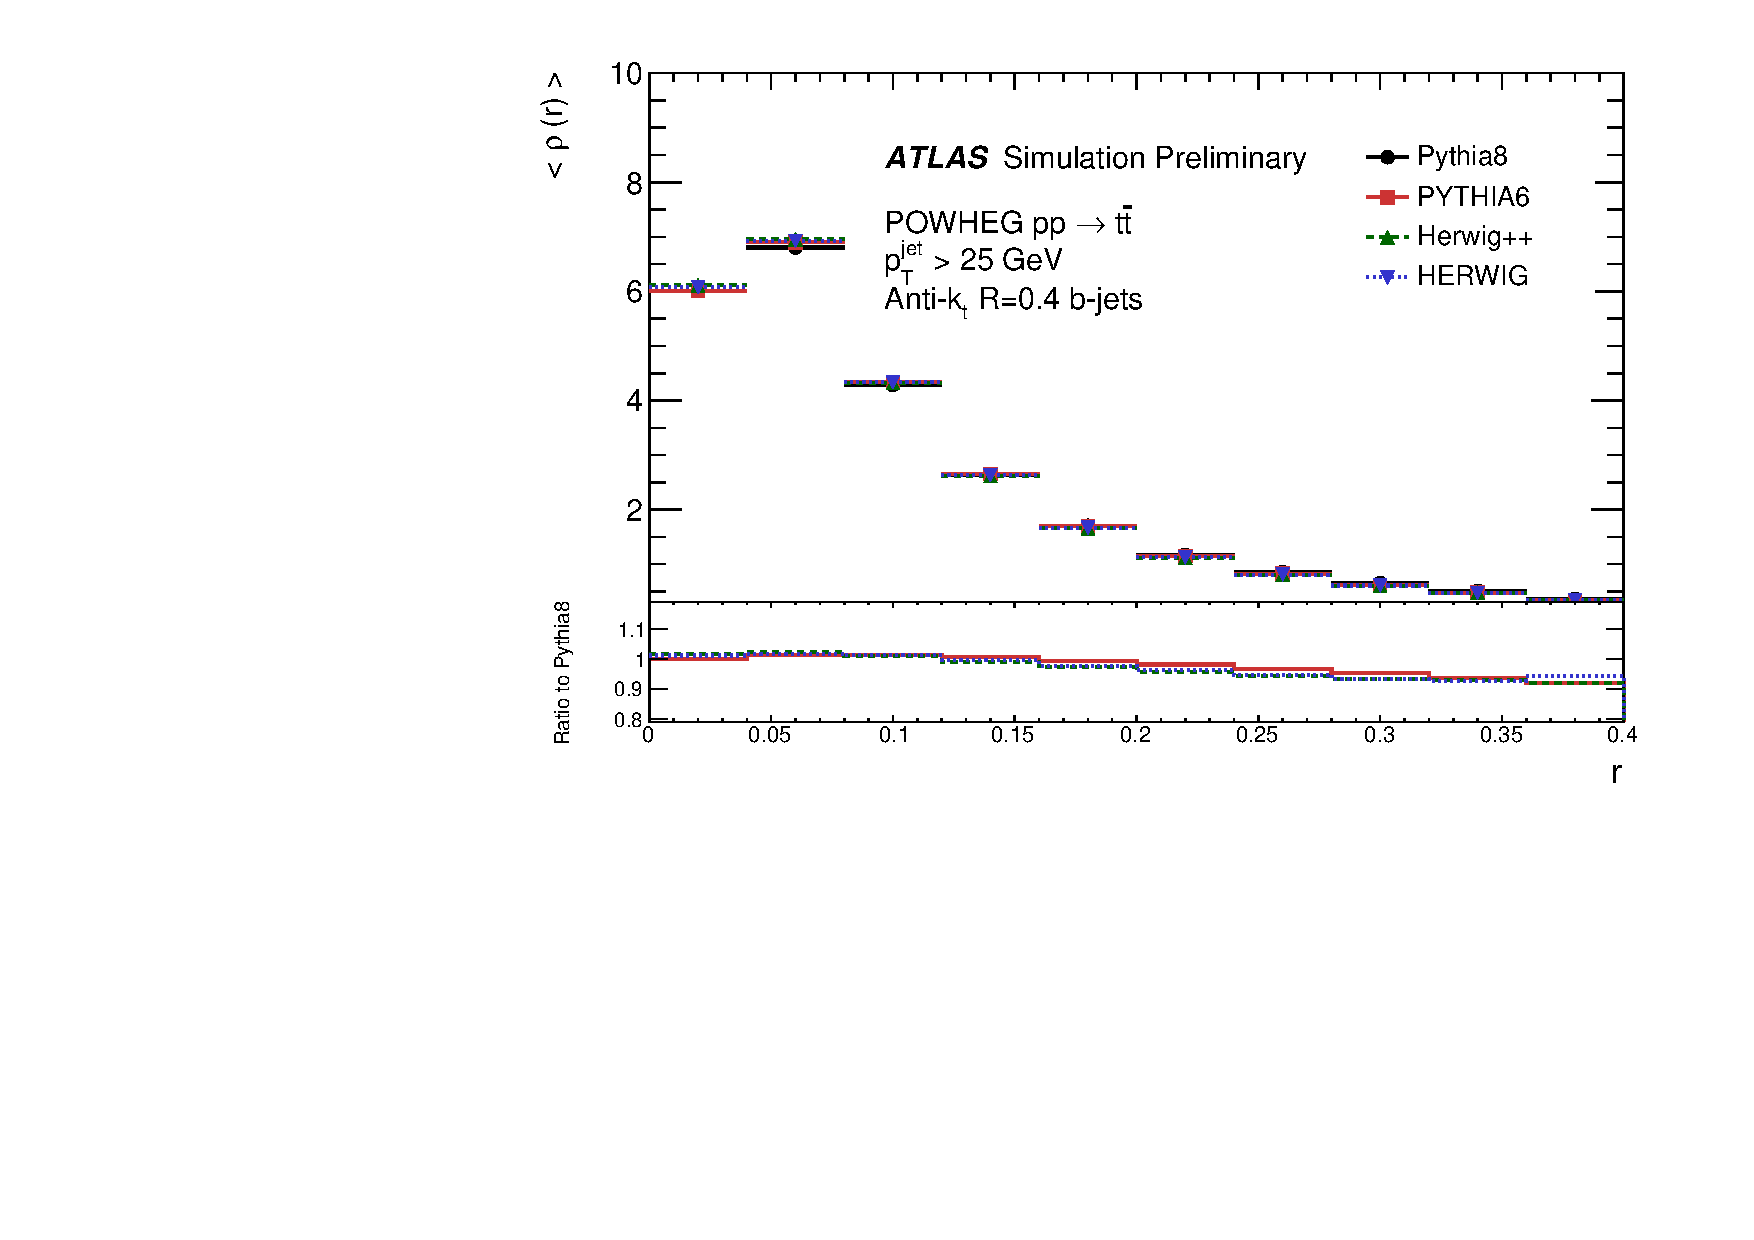
\includegraphics[width=\textwidth]{evtgen/figures/Frag/Top/SingleB/Rho.pdf}
\end{subfigure}
\begin{subfigure}[]{0.45\textwidth}
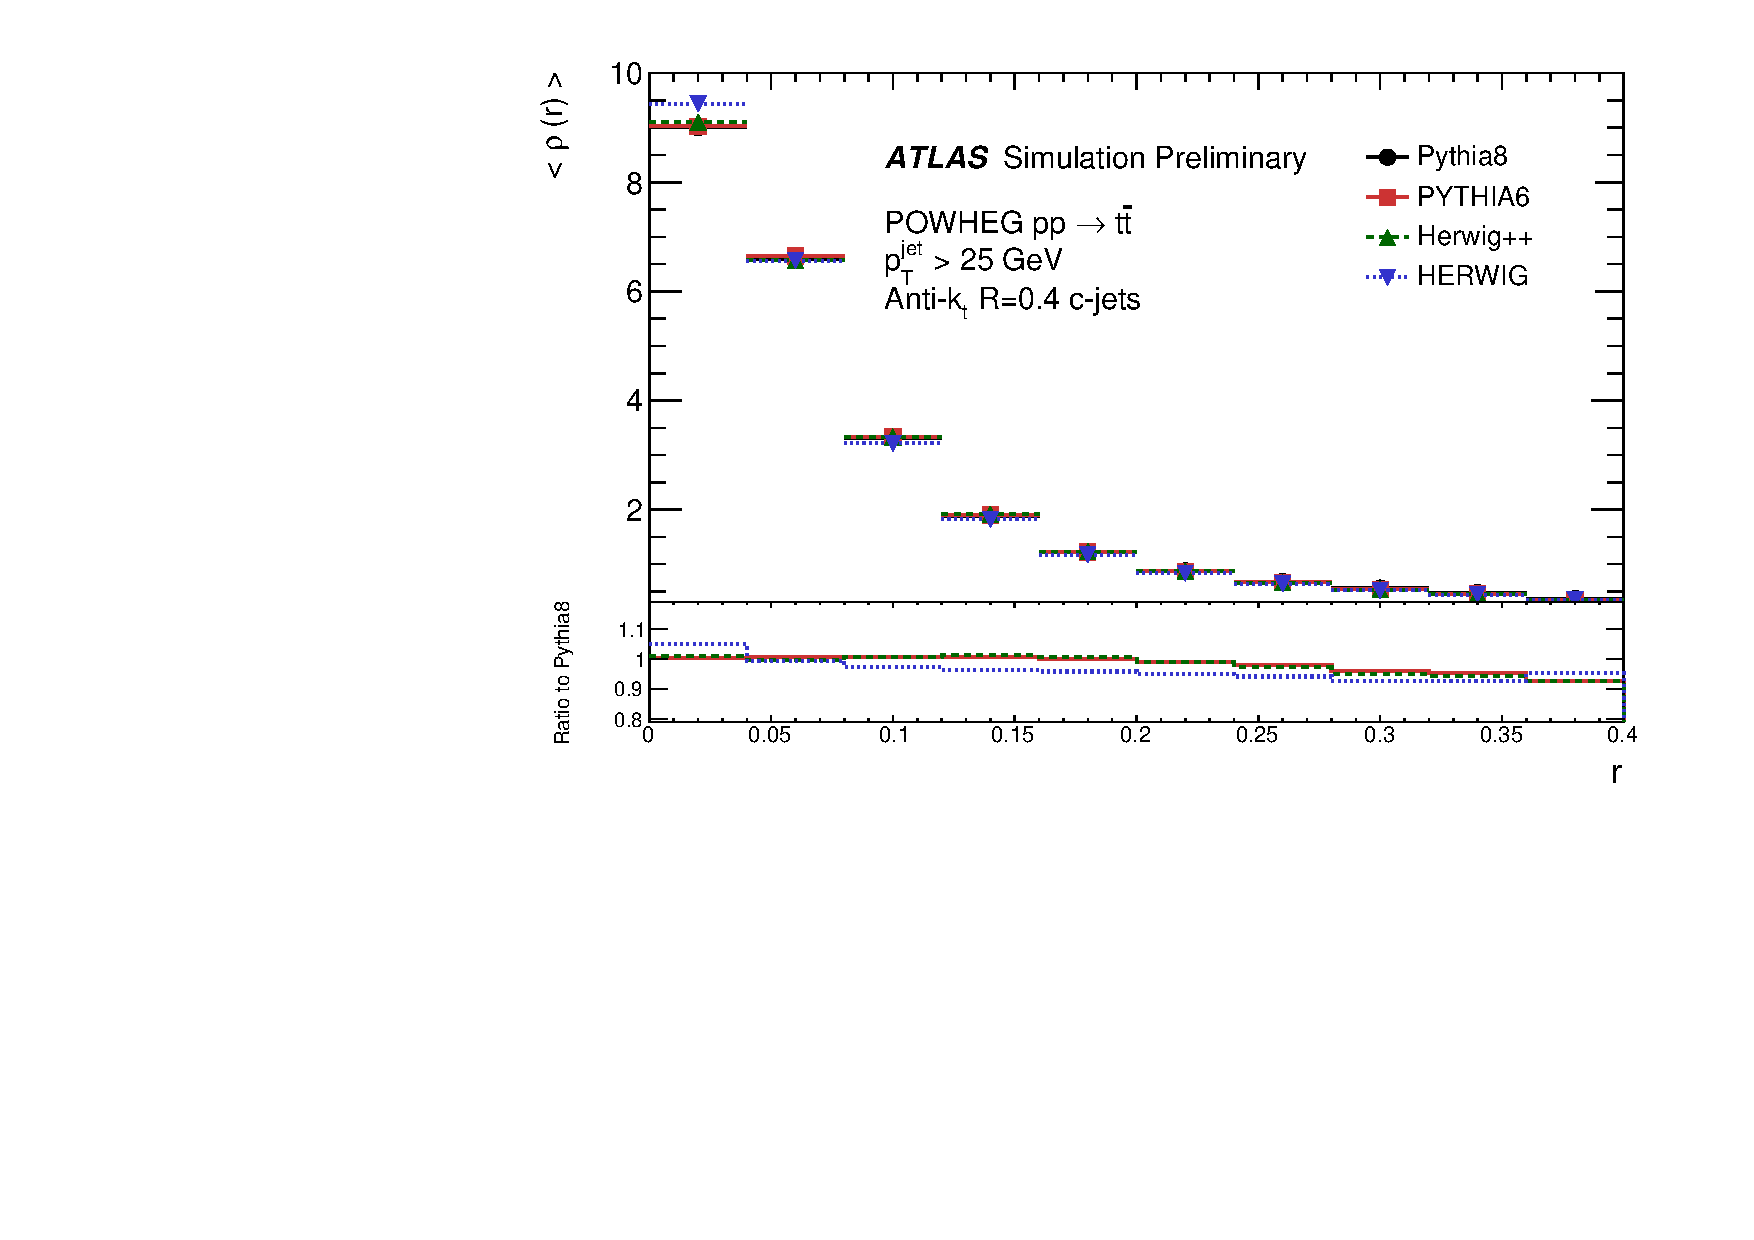
\includegraphics[width=\textwidth]{evtgen/figures/Frag/Top/SingleC/Rho.pdf}
\end{subfigure}
\caption{The differential jet shape $\rho(r)$ distribution for 
(a)~$b$-jets and (b)~$c$-jets in \PowHeg\
\ttbar\ samples where  \PythiaE, \Pythia, \Herwigpp\ and \Herwig\ have been used 
for the parton shower, hadronization and underlying event modeling. }
\label{fig:trho}
\end{figure}


\begin{figure}
\centering
\begin{subfigure}[]{0.45\textwidth}
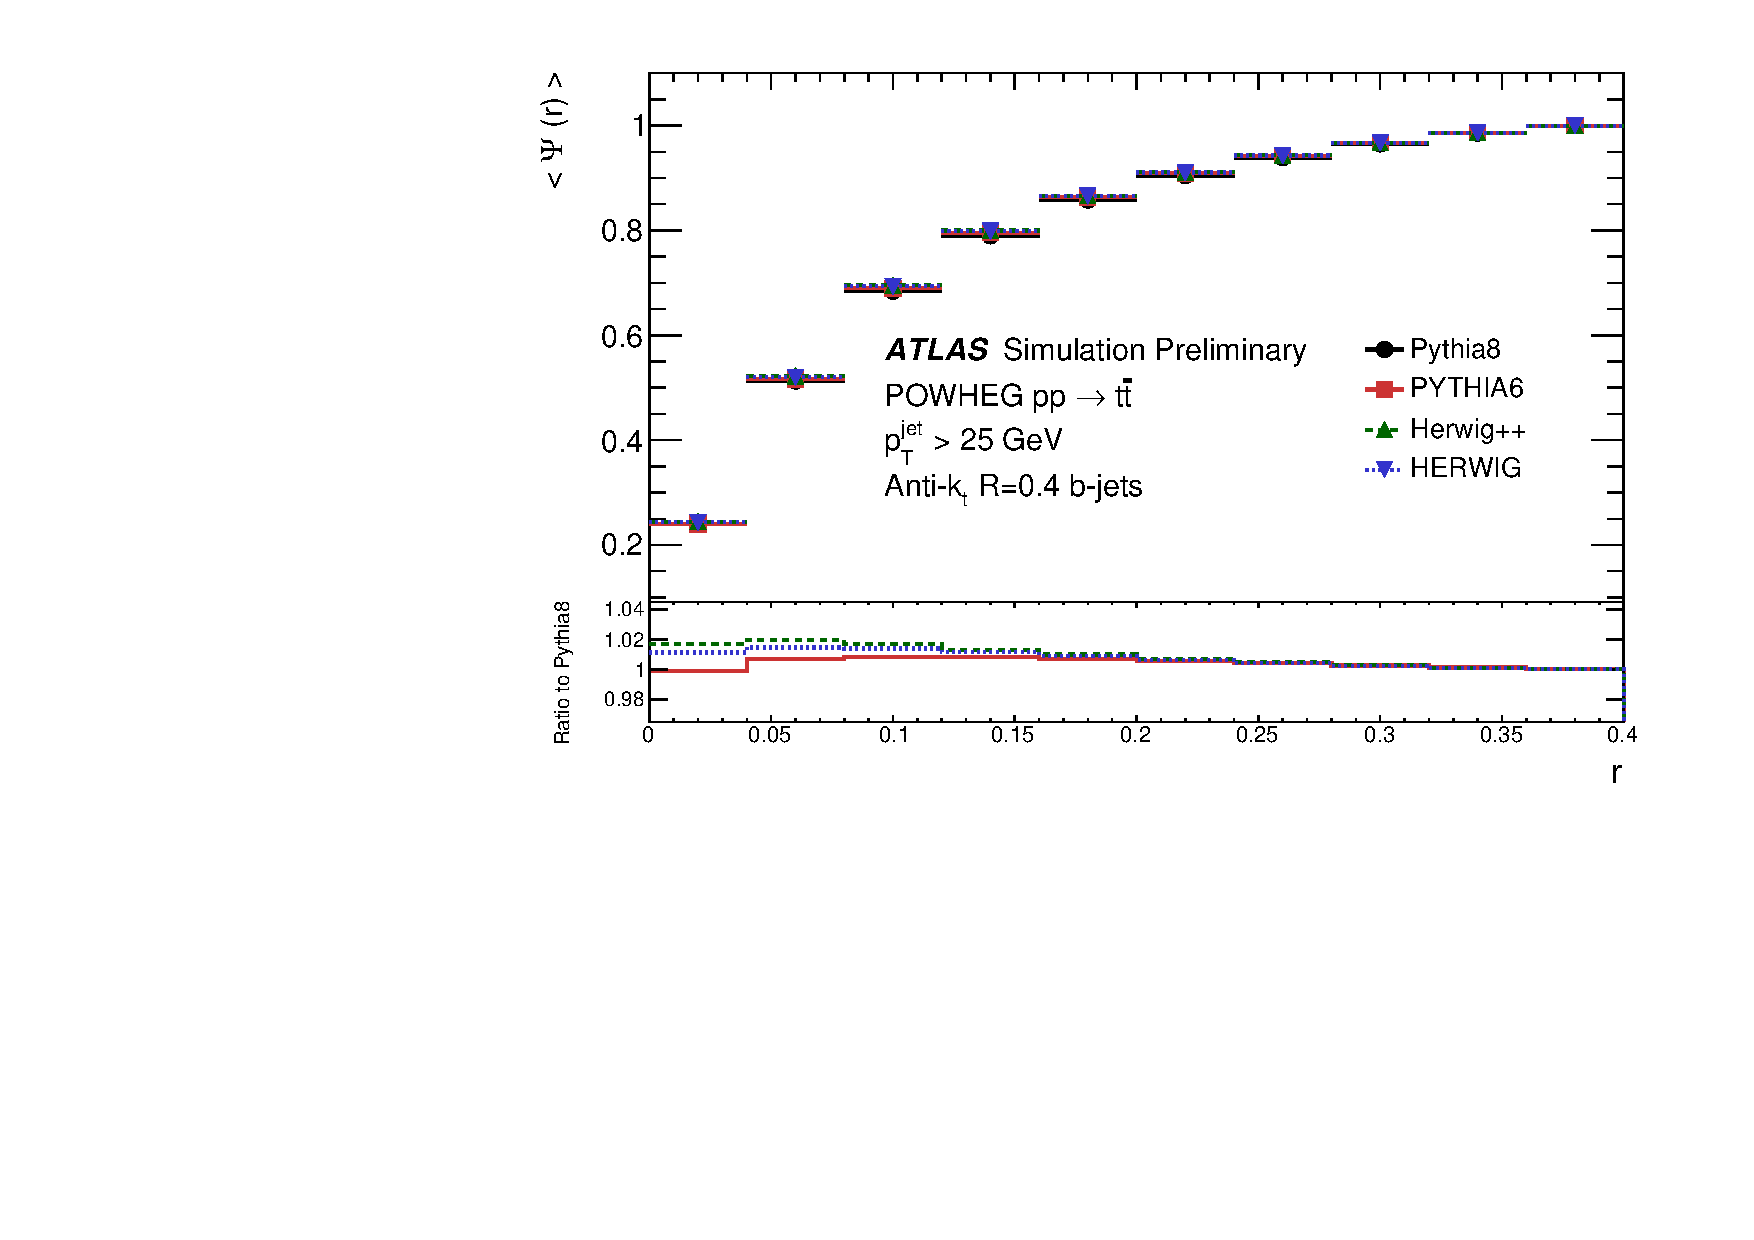
\includegraphics[width=\textwidth]{evtgen/figures/Frag/Top/SingleB/PsiVariableR.pdf}
\end{subfigure}
\begin{subfigure}[]{0.45\textwidth}
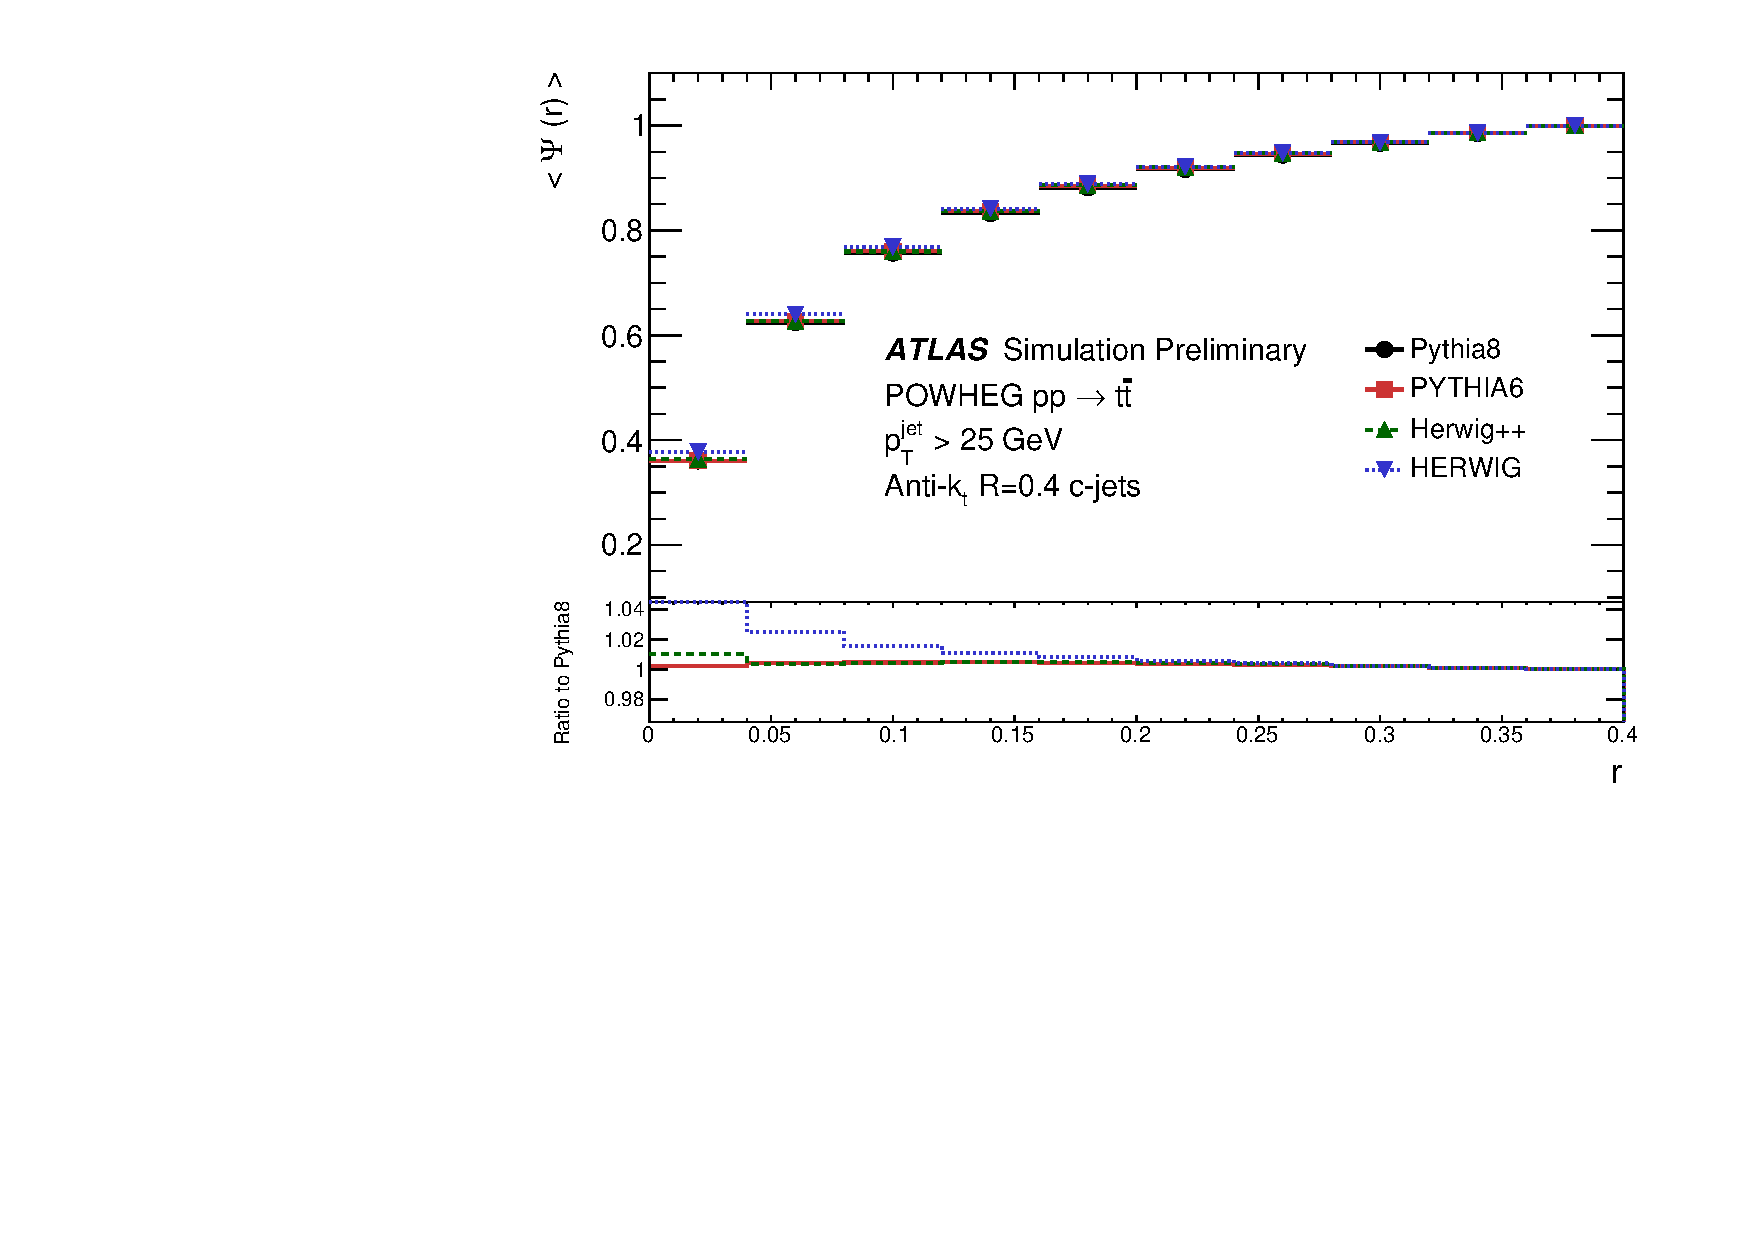
\includegraphics[width=\textwidth]{evtgen/figures/Frag/Top/SingleC/PsiVariableR.pdf}
\end{subfigure}
\caption{The integral jet shape 
$\Psi \left( r, R=0.4 \right ) \equiv  \Sigma p_T \left(0, r \right) \ \sum p_T \left(0, R \right) $ 
distribution for 
(a)~$b$-jets and (b)~$c$-jets in \PowHeg\
\ttbar\ samples where  \PythiaE, \Pythia, \Herwigpp\ and \Herwig\ have been used 
for the parton shower, hadronization and underlying event modeling. The legend includes the value and error of the mean of each distribution.}
\label{fig:tpsi}
\end{figure}



\begin{figure}
\centering
\begin{subfigure}[]{0.45\textwidth}
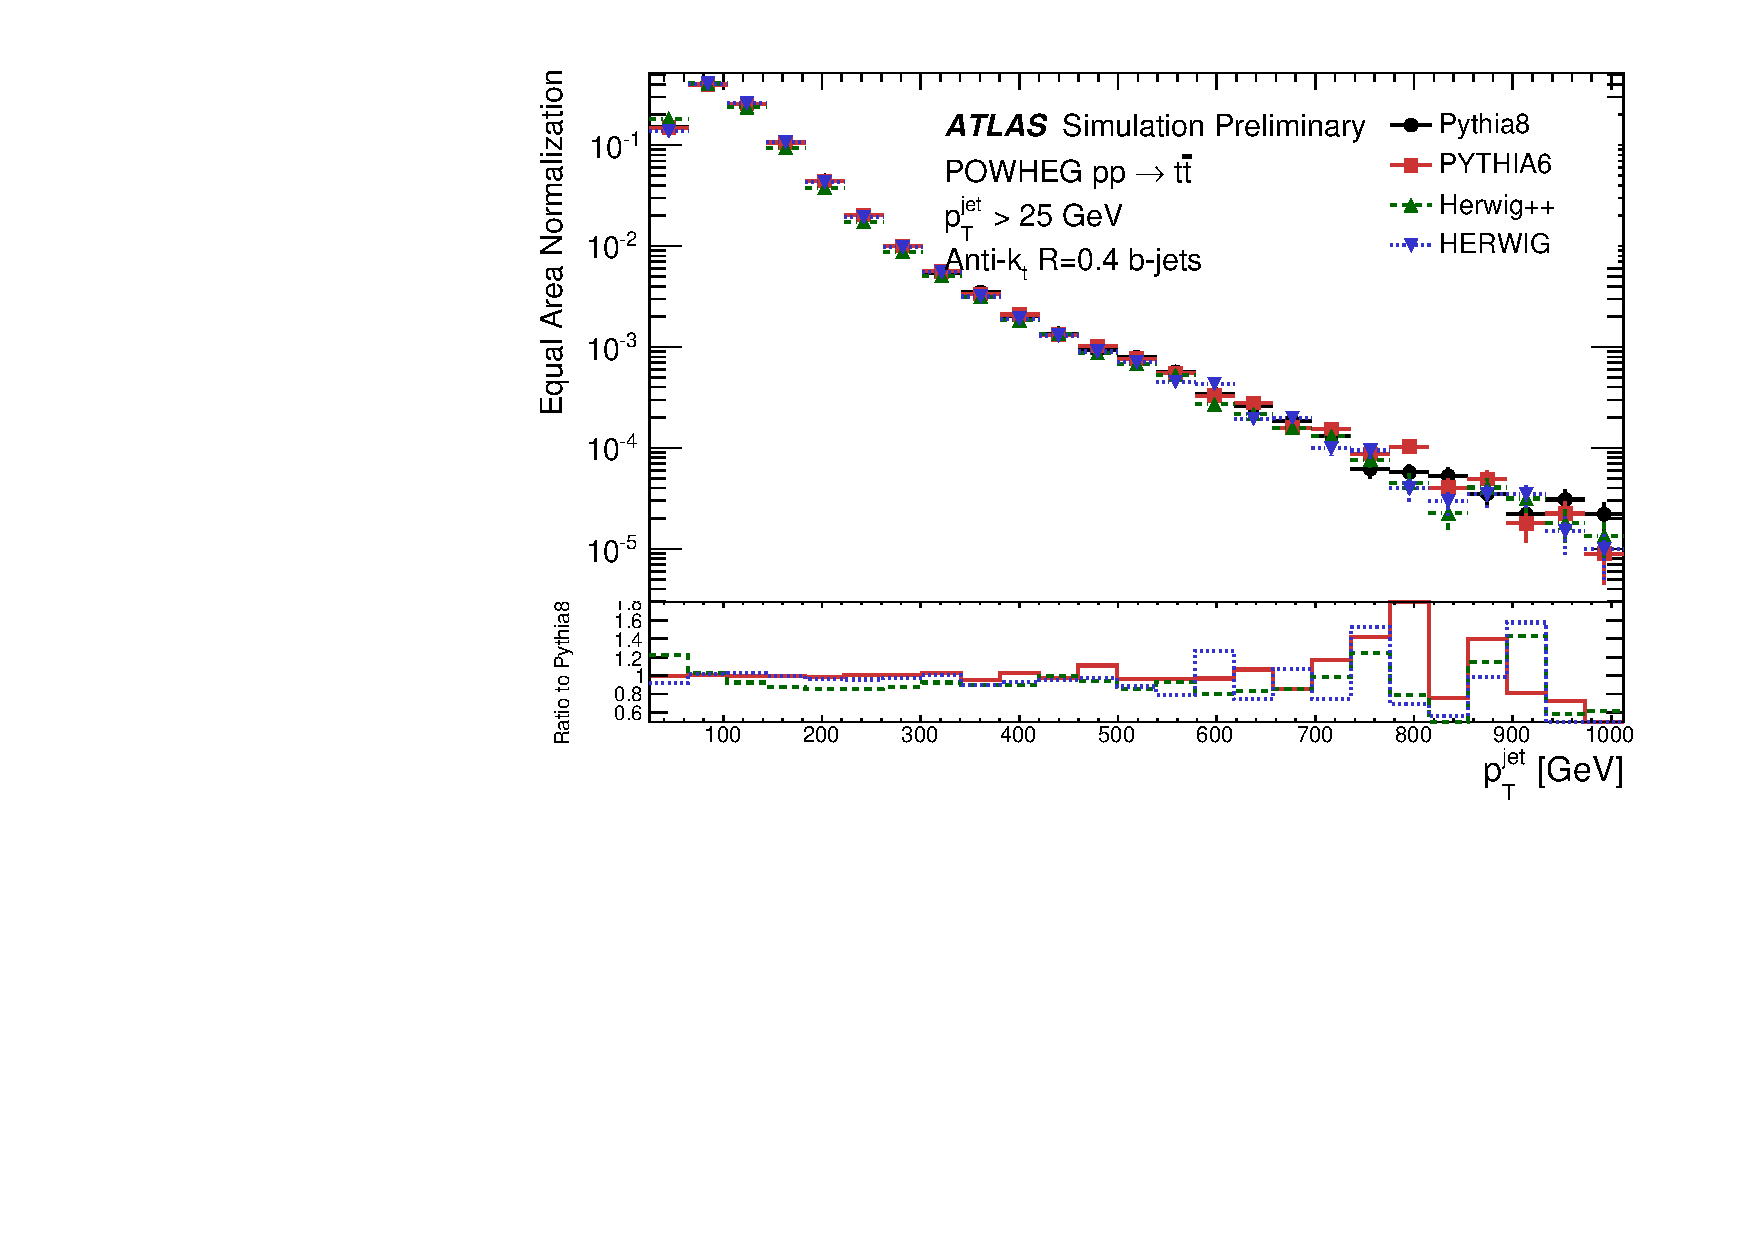
\includegraphics[width=\textwidth]{evtgen/figures/Frag/Top/SingleB/h_JetpT.pdf}
\end{subfigure}
\begin{subfigure}[]{0.45\textwidth}
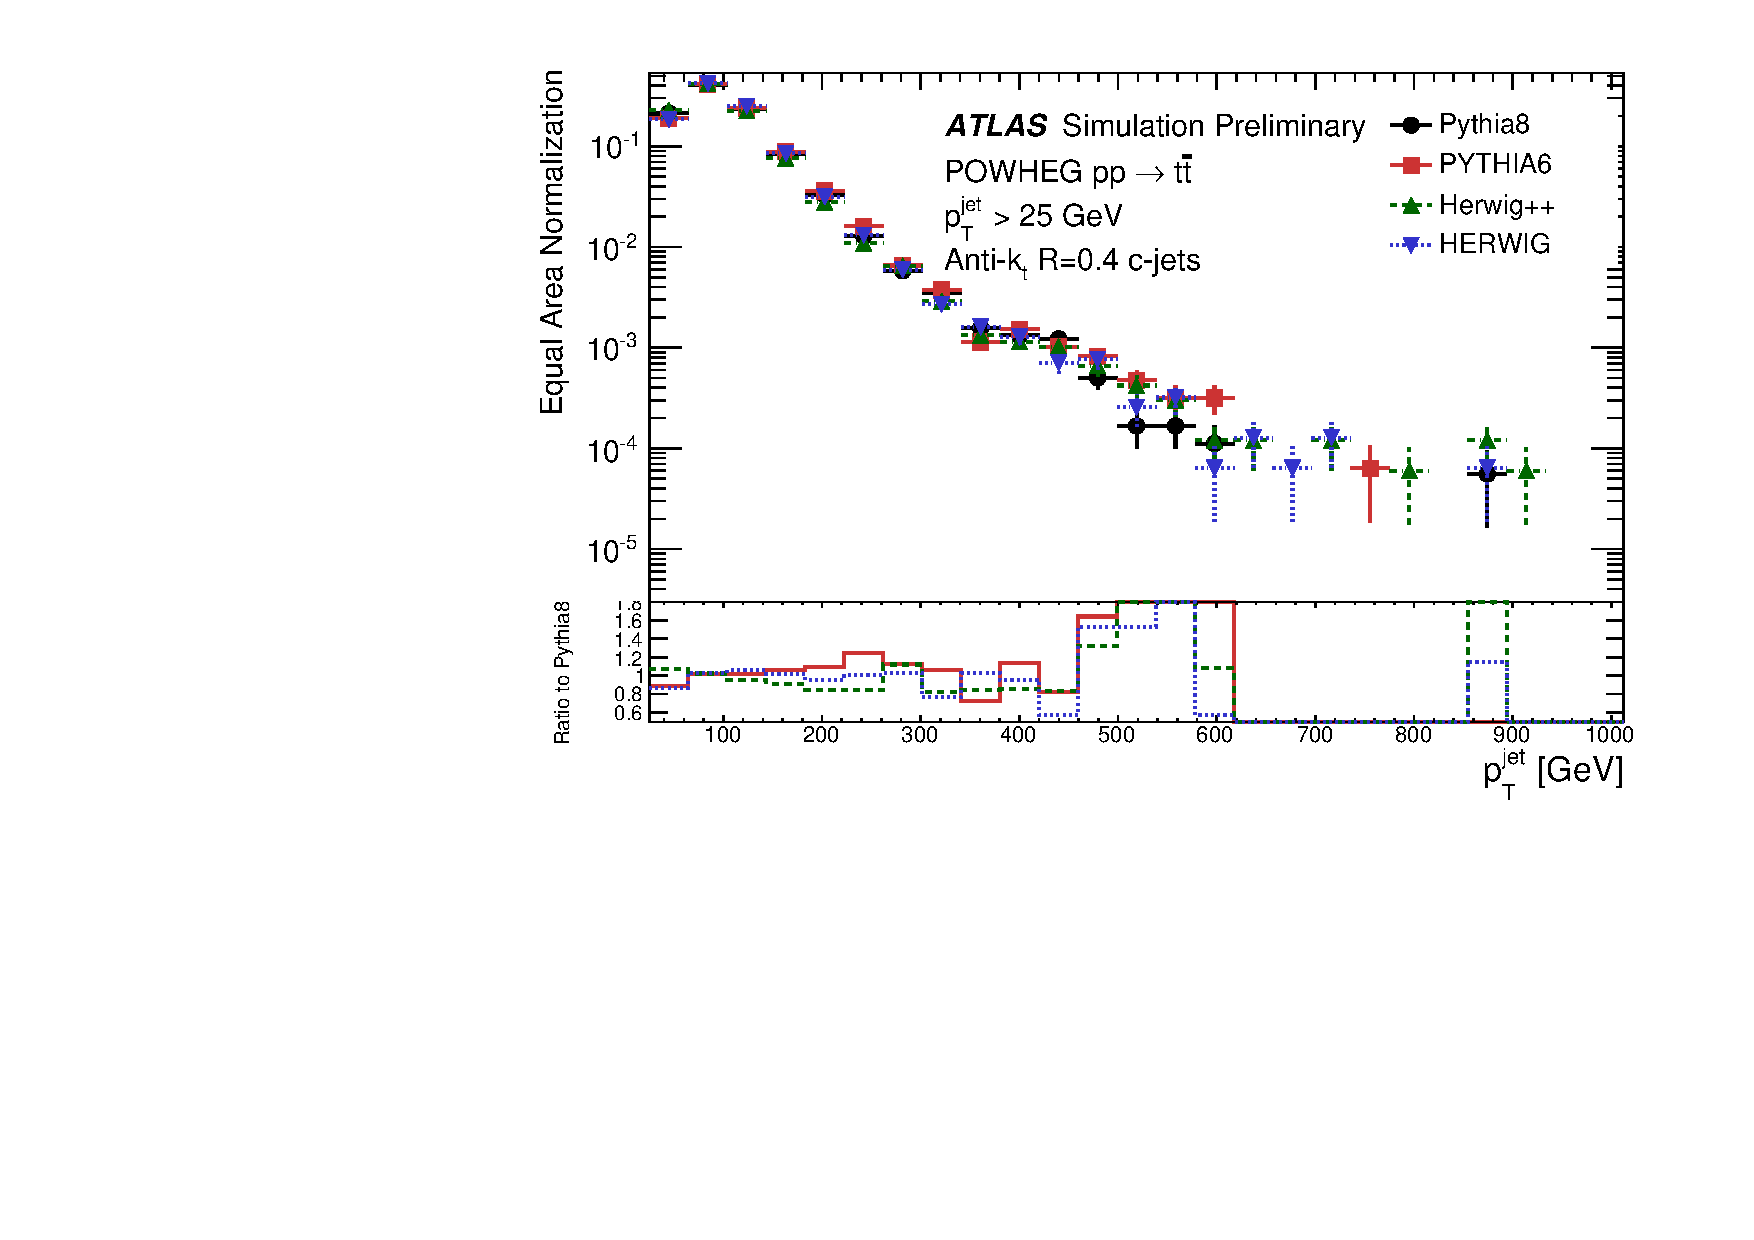
\includegraphics[width=\textwidth]{evtgen/figures/Frag/Top/SingleC/h_JetpT.pdf}
\end{subfigure}
\caption{The \ptJet\ distribution for 
(a)~$b$-jets and (b)~$c$-jets in \PowHeg\
\ttbar\ samples where  \PythiaE, \Pythia, \Herwigpp\ and \Herwig\ have been used 
for the parton shower, hadronization and underlying event modeling.}
\label{fig:tjpt}
\end{figure}

\begin{figure}
\centering
\begin{subfigure}[]{0.45\textwidth}
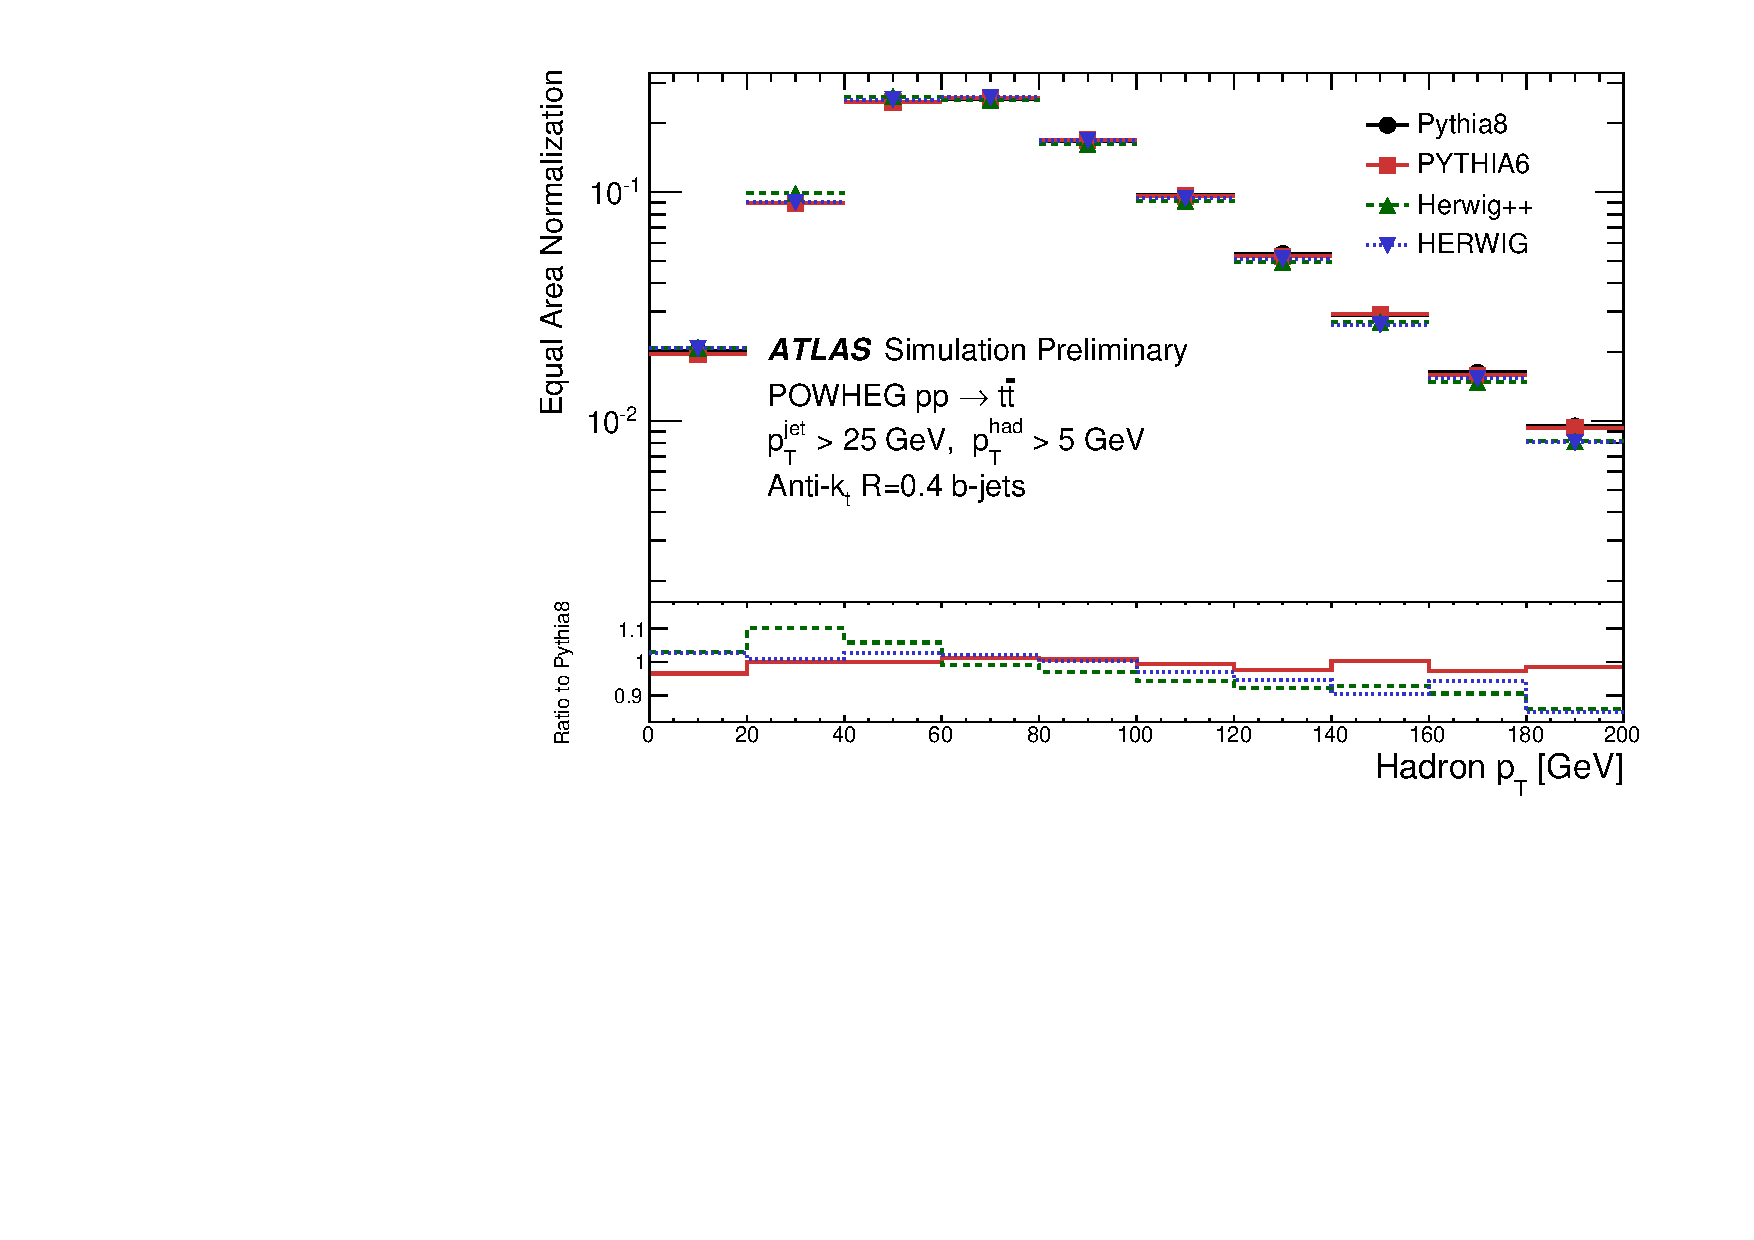
\includegraphics[width=\textwidth]{evtgen/figures/Frag/Top/SingleB/h_HardHadpT.pdf}
\end{subfigure}
\begin{subfigure}[]{0.45\textwidth}
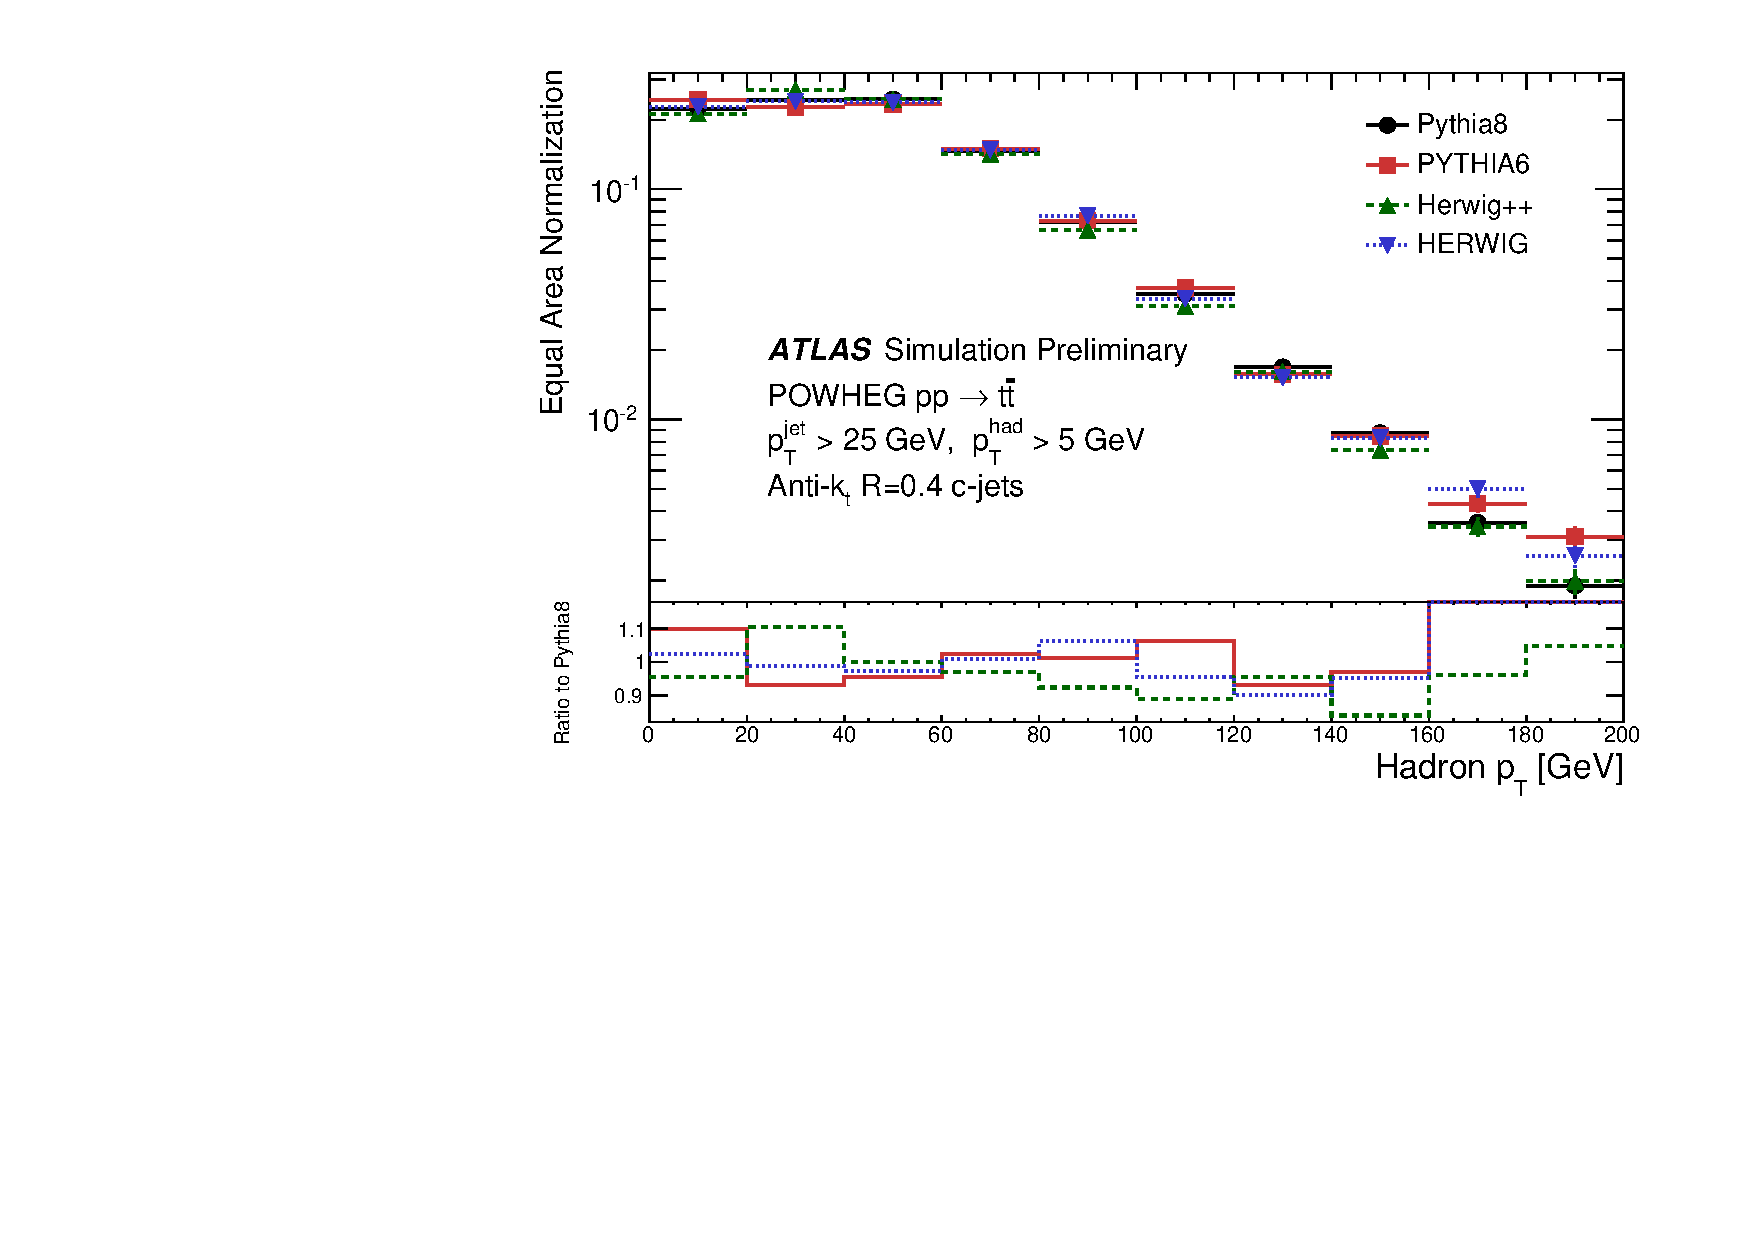
\includegraphics[width=\textwidth]{evtgen/figures/Frag/Top/SingleC/h_HardHadpT.pdf}
\end{subfigure}
\caption{The \ptHad\ distribution for 
(a)~$b$-jets and (b)~$c$-jets in \PowHeg\
\ttbar\ samples where  \PythiaE, \Pythia, \Herwigpp\ and \Herwig\ have been used 
for the parton shower, hadronization and underlying event modeling.}
\label{fig:thadpt}
\end{figure}


\begin{figure}
\centering
 \begin{subfigure}[]{0.45\textwidth}
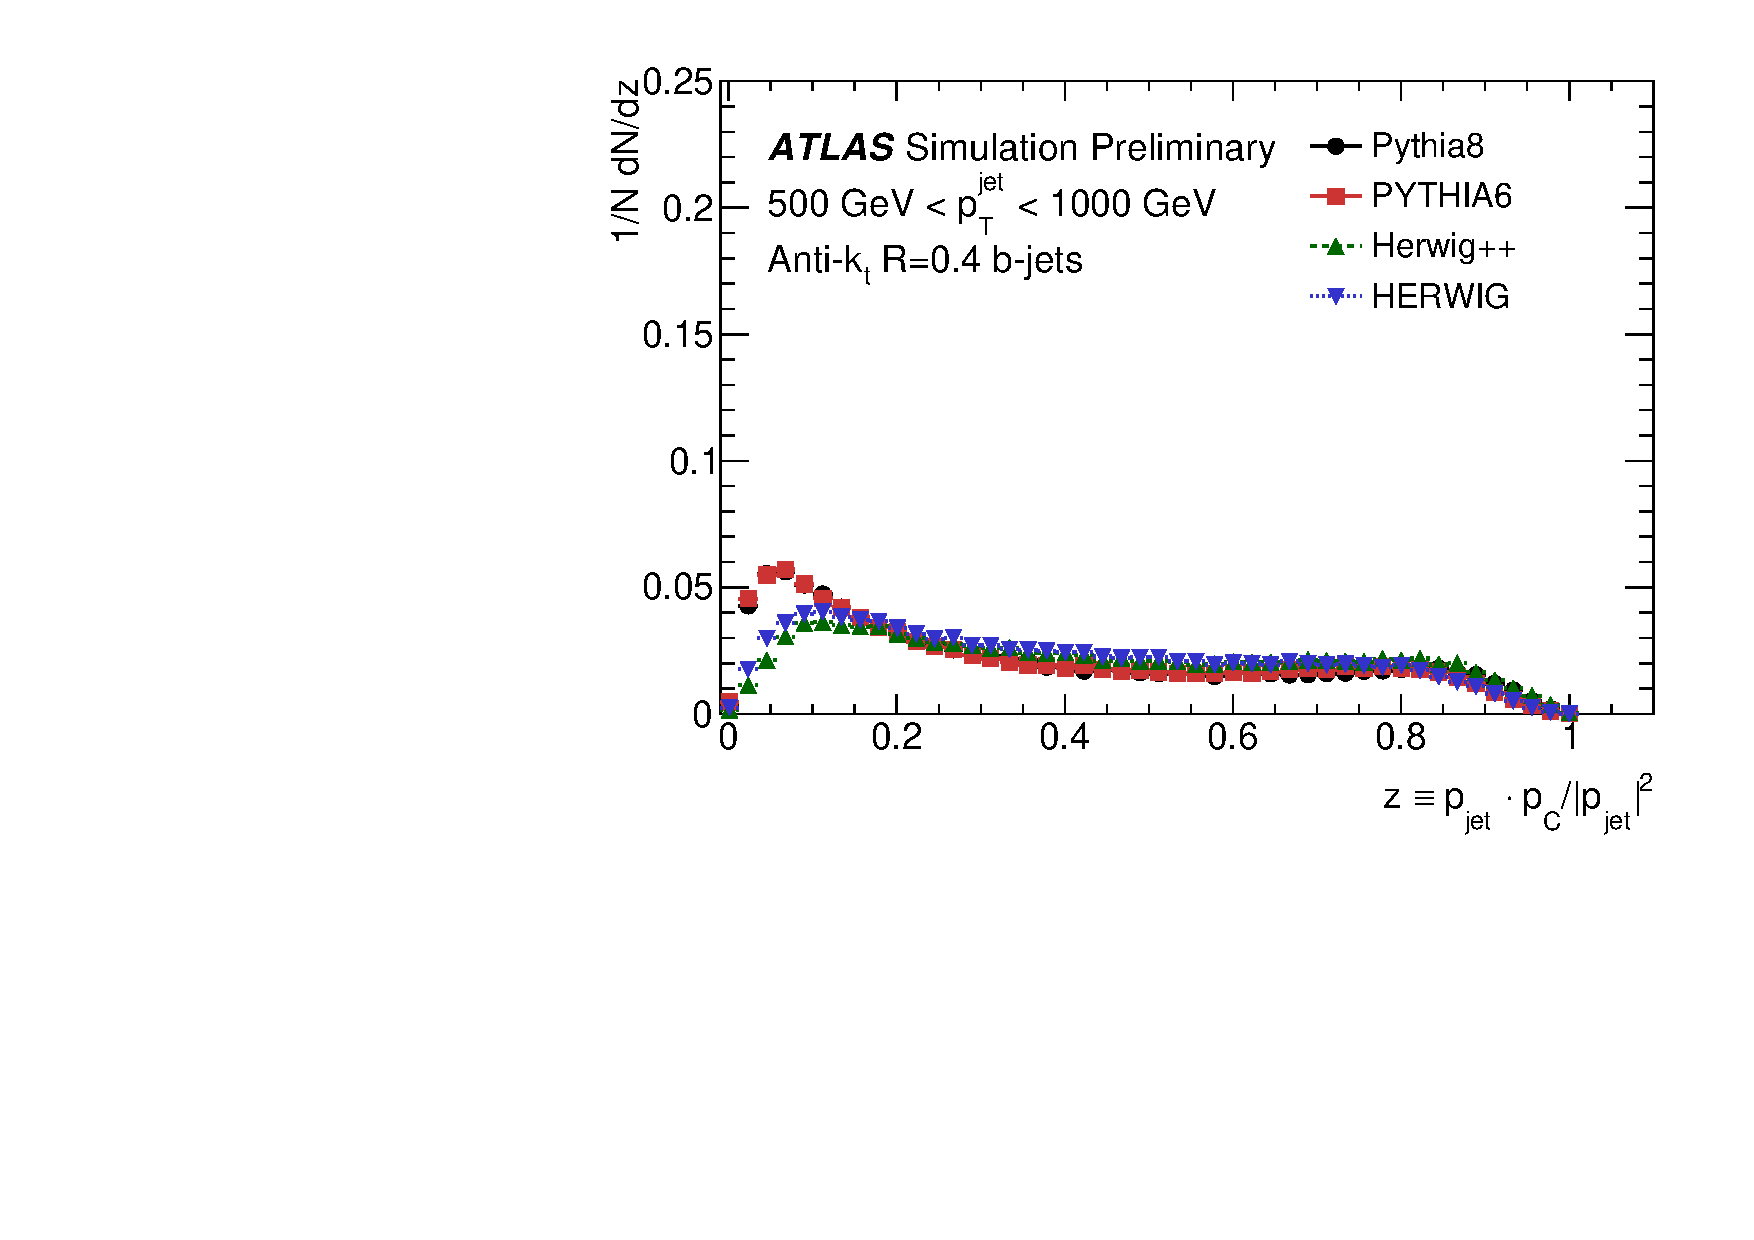
\includegraphics[width=\textwidth]{evtgen/figures/Frag/Jz4/WithIsolation/h_BFrag.pdf}
\end{subfigure}
 \begin{subfigure}[]{0.45\textwidth}
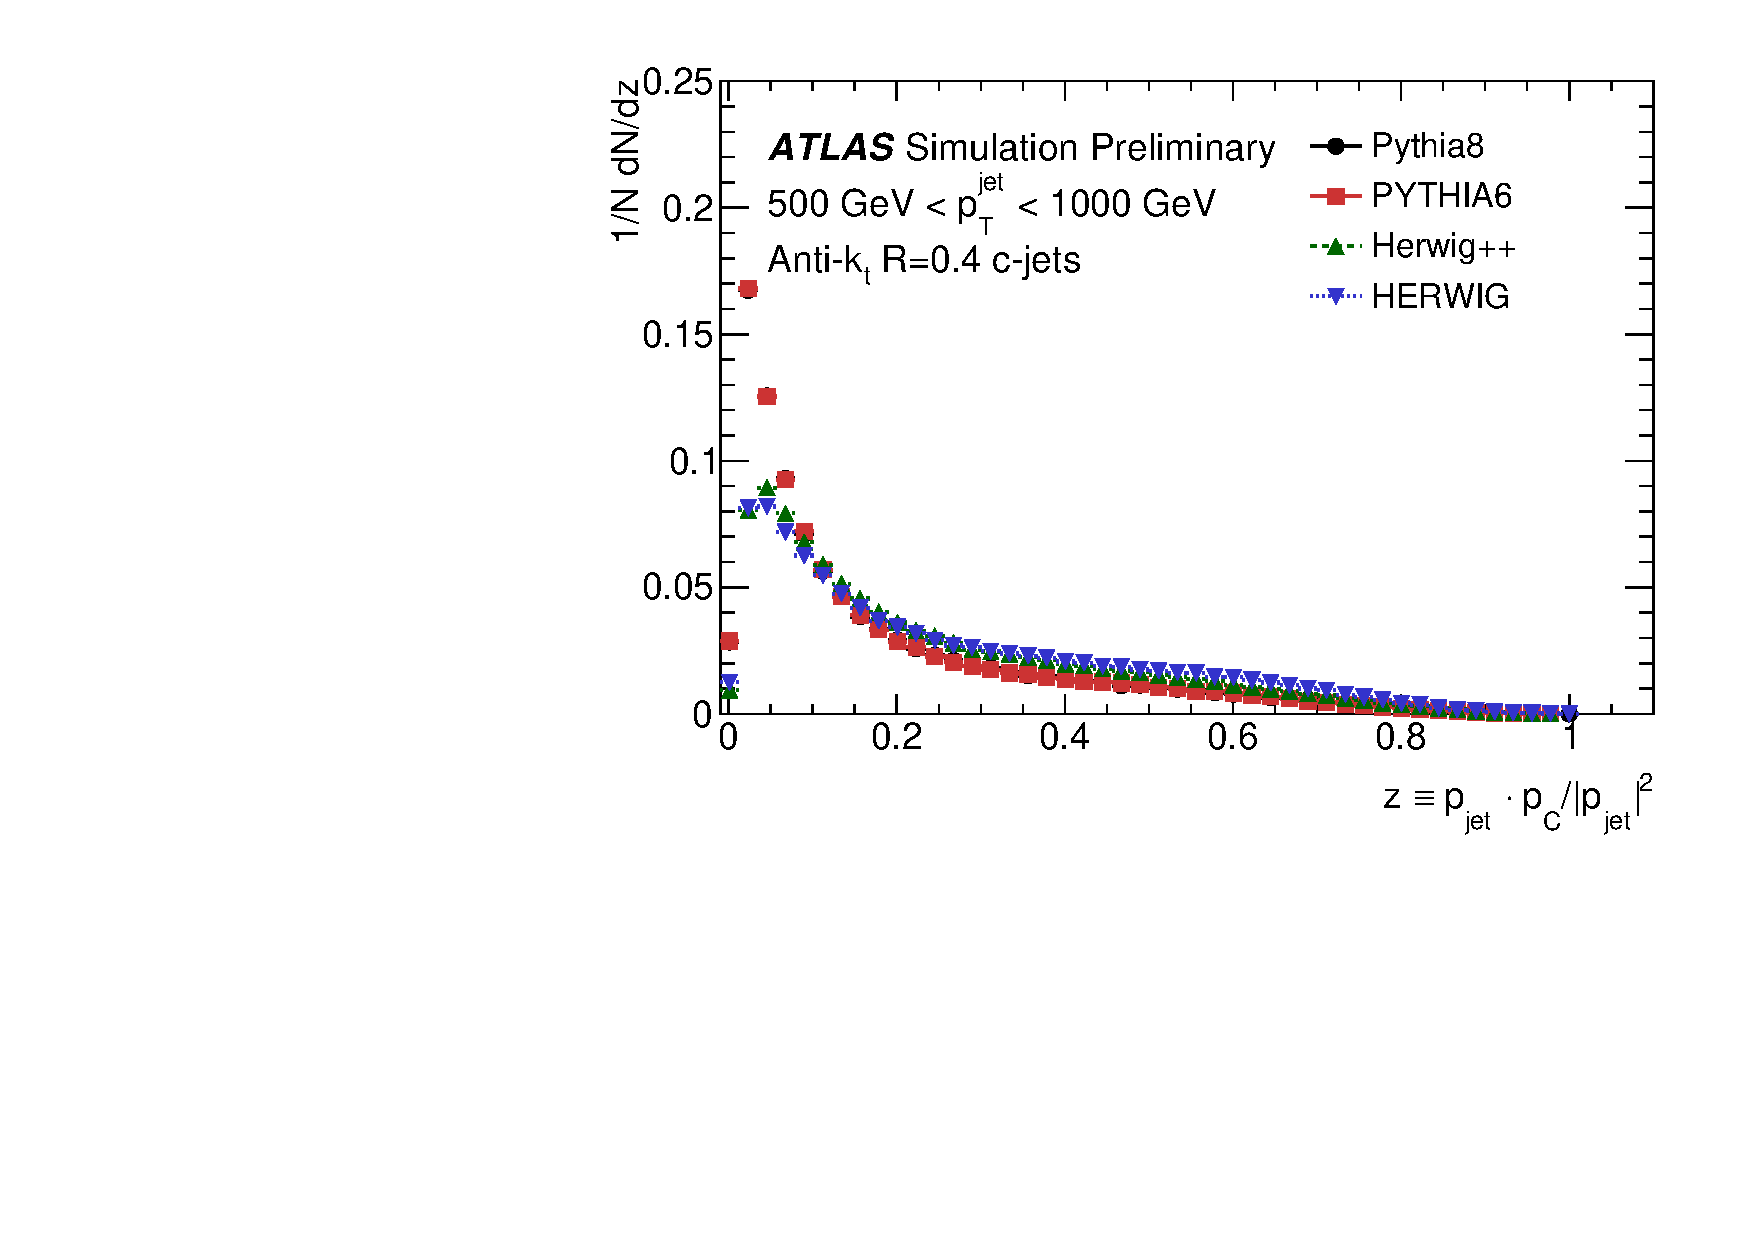
\includegraphics[width=\textwidth]{evtgen/figures/Frag/Jz4/WithIsolation/h_CFrag.pdf}
\end{subfigure}
  \begin{subfigure}[]{0.45\textwidth}
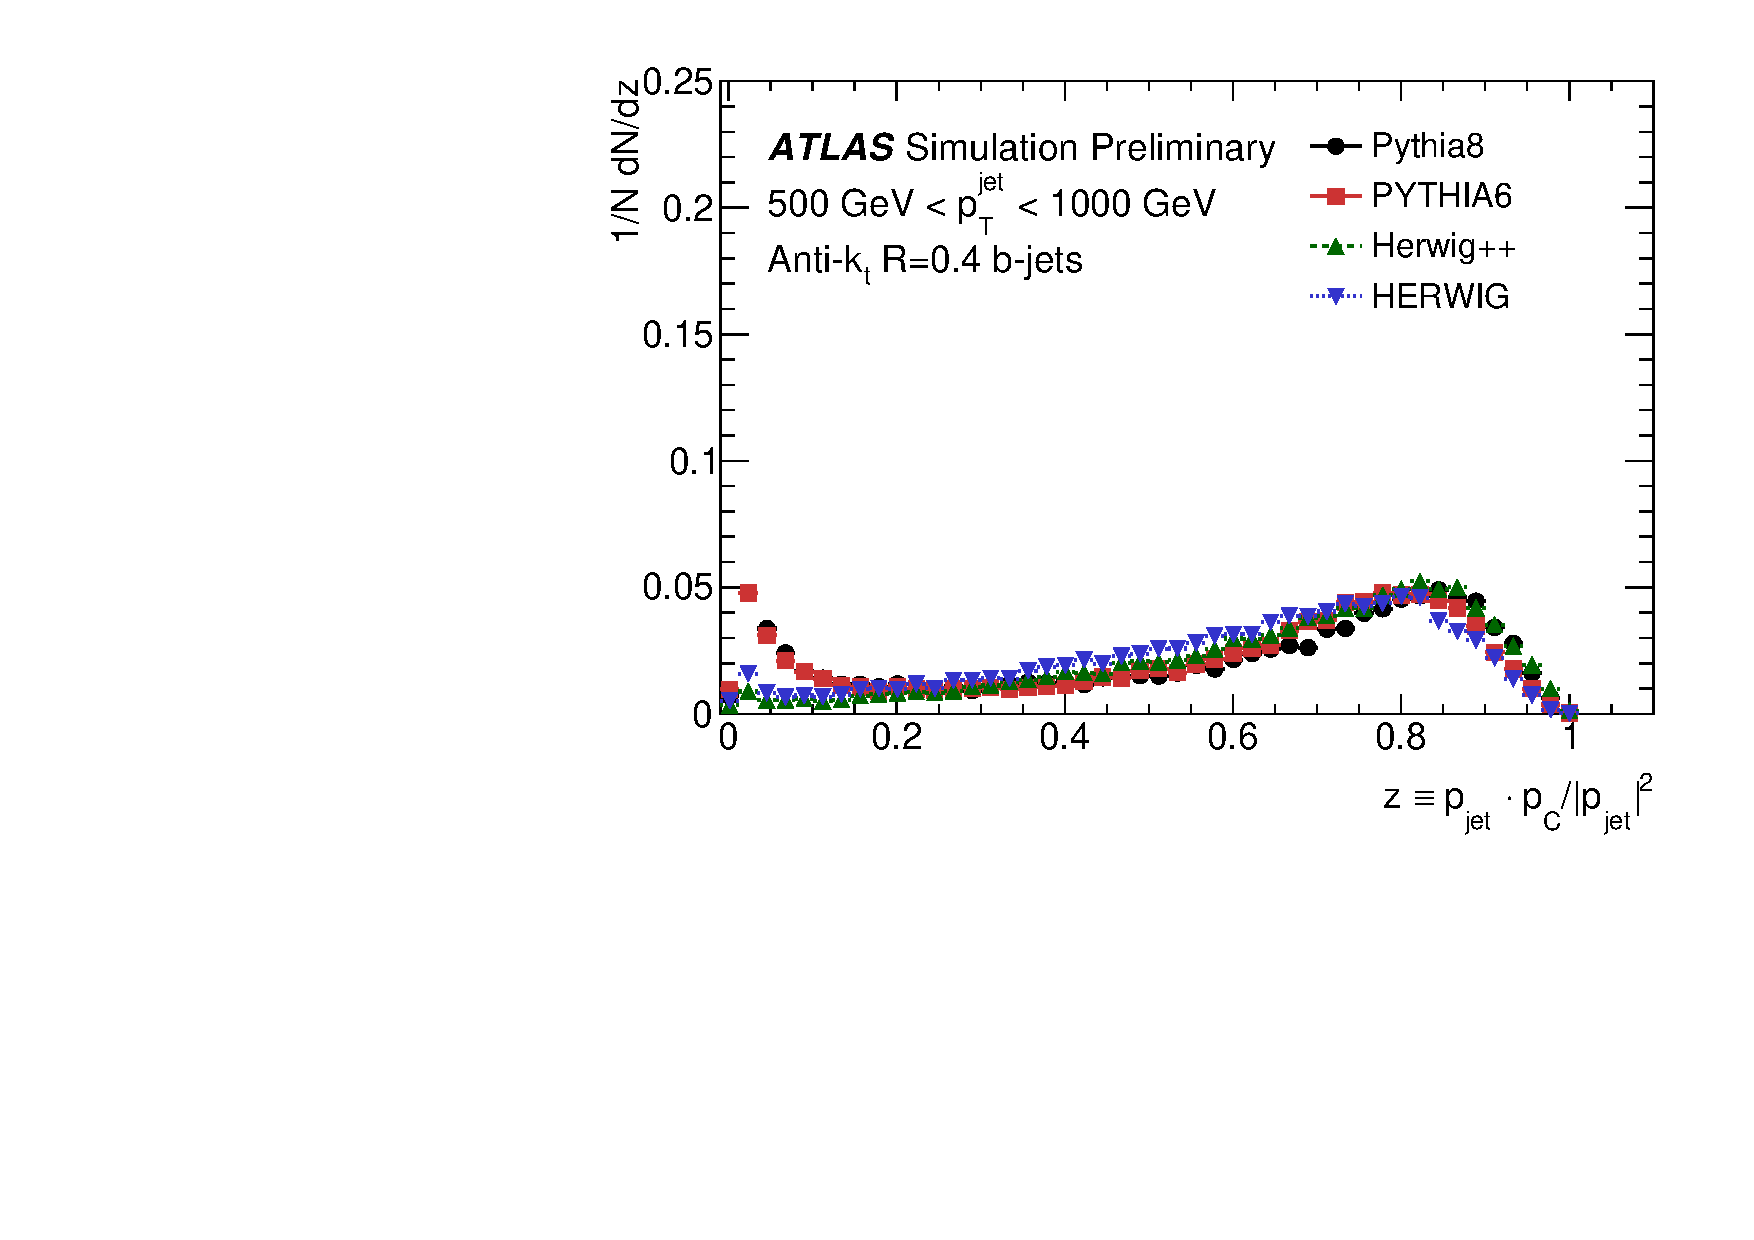
\includegraphics[width=\textwidth]{evtgen/figures/Frag/Jz4/WithIsolation/h_BFrag_SingleHad.pdf}
\end{subfigure}
 \begin{subfigure}[]{0.45\textwidth}
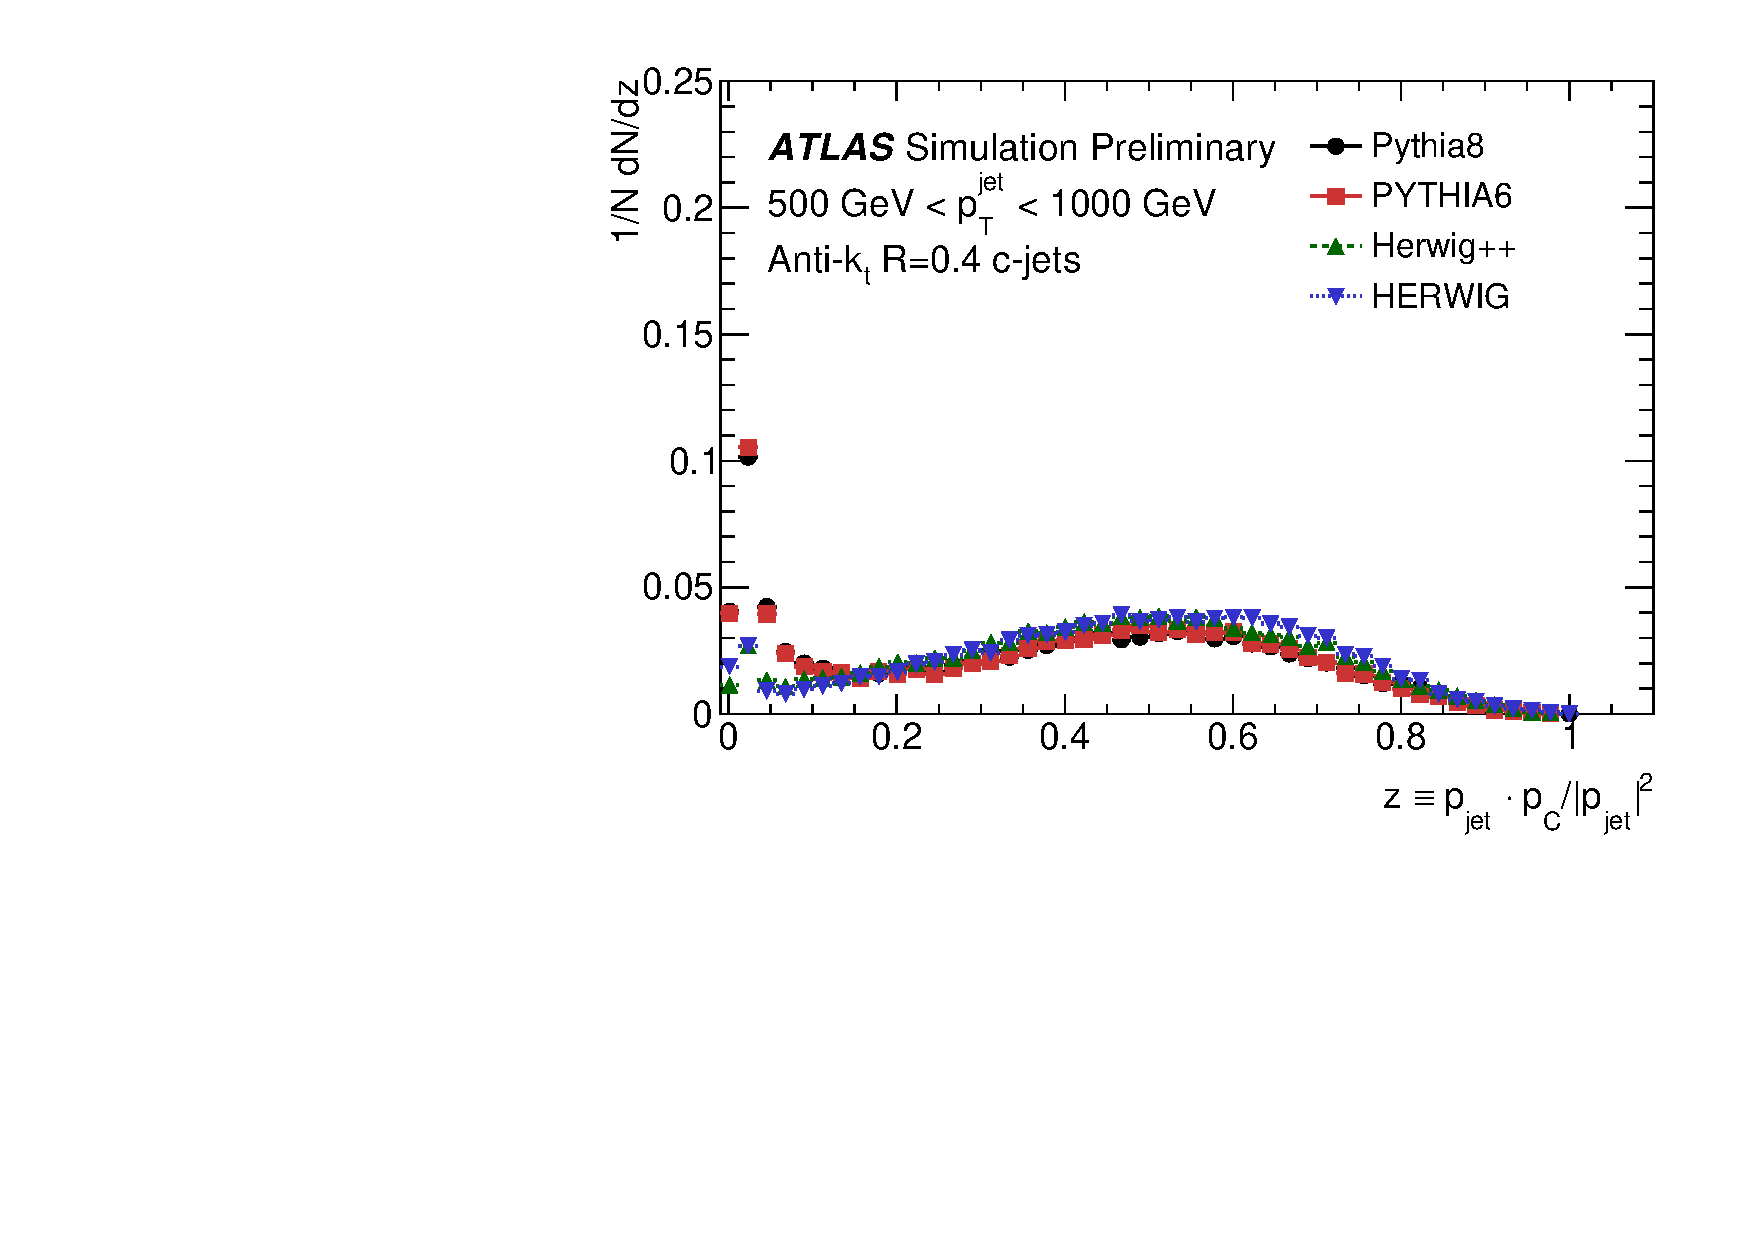
\includegraphics[width=\textwidth]{evtgen/figures/Frag/Jz4/WithIsolation/h_CFrag_SingleHad.pdf}
\end{subfigure}

\caption{The fragmentation function for (a)~$b$-jets and (b)~$c$-jets in the 
high \pT\ jet sample and for the subset
of (c)~$b$-jets and (d)~$c$-jets containing exactly one heavy flavor hadron.
}
\label{fig:jz4frag}
\end{figure}
\begin{table}
\subfloat{
\centering
All jets
\newline
\begin{tabular}{|r|r|r|}
\hline
\multicolumn{3}{l}{All jets} \\
\hline
Generator & $p_{jet} \cdot p_{B}/p_{jet}^2$  & $p_{jet} \cdot p_{C}/p_{jet}^2$ \\
\hline
 \PythiaE & $0.3683 \pm 0.0012$   & $0.1853 \pm 0.0004$    \\
 \Pythia & $0.3633 \pm 0.0010$  & $0.1841 \pm 0.0004$ \\
 \Herwigpp & $0.4356 \pm 0.0011$   & $0.2442 \pm 0.0005$    \\
 \Herwig  & $0.3984 \pm 0.0011$   & $0.2614 \pm 0.0006$   \\
\hline
\end{tabular}
}
\hfill
\subfloat{
\centering
\begin{tabular}{|r|r|r|}
\hline
\multicolumn{3}{l}{Heavy flavor hadron jets} \\
\hline
Generator & $p_{jet} \cdot p_{B}/p_{jet}^2$  & $p_{jet} \cdot p_{C}/p_{jet}^2$ \\
\hline
 \PythiaE & $0.5747 \pm 0.0022$  & $0.3790 \pm 0.0018$   \\
 \Pythia & $0.5696 \pm 0.0019$  & $0.3787 \pm 0.0016$ \\
 \Herwigpp & $0.6473 \pm 0.0017$  &$0.4549 \pm 0.0015$   \\
 \Herwig  & $0.5953 \pm 0.0017$  & $0.4674 \pm 0.0015$   \\
\hline
\end{tabular}
}
\caption{The mean fragmentation function for (a)~$b$-jets and $c$-jets in the 
high \pT~jet sample and for the subset
of (b)~$b$-jets and ~$c$-jets 
satisfying the additional requirement that there be no other weakly decaying
heavy flavor hadron with $\pt>5.0$~\GeV\ within a cone $\Delta R=1$ of the jet.}
\label{t:jz4frag}
\end{table}
The differential jet shape $\rho (r)$ in an annulus of inner radius $r-\Delta r /2$ and outer radius $r+\Delta r /2$ from the axis~\footnote{The jet axis is defined to be the direction of the momentum vector of the jet from the \antiktfour\ algorithm.} of a given jet is defined as

$$
\rho(r) = \frac{1}{\Delta r} \frac{p_T \left(r-\Delta r /2, r+\Delta r /2 \right)}{p_T \left(0, R \right)}
$$ 
\noindent
Here $\Delta r = 0.04$ is the width of the annulus, $r$, such that $\Delta r /2 \leq r \leq R - \Delta r /2$ is the distance to the jet axis in the $\eta-\phi$ plane and $p_T(r_1, r_2)$ is the scalar sum of the $p_T$ of the jet constituents with radii between $r_1$ and $r_2$. Figure~\ref{fig:trho} shows the distribution of the variable $\rho(r)$. 
ATLAS results for \ttbar\ production at 7~\TeV\ indicate that \PowHeg\ with \Pythia\ for the parton shower give
good agreement with the data for this variable~\cite{Aad:2013fba}. No experimental results are currently available at 8~\TeV.

The integrated jet shape in a cone of radius $r<R$ around the jet axis is defined as the cumulative distribution for $\rho(r)$, i.e.

$$
\Psi(r) \equiv \frac{p_T \left(0, r \right)}{p_T \left(0, R \right)},\; 0 \leq r \leq R 
$$
\noindent
which satisfies $\Psi(r = R) = 1$.
Figure~\ref{fig:tpsi} shows the distribution of $\Psi(r)$. For each of these jet shapes, differences between the 
generators are small. The fact that \Herwigpp\ (\Herwig) $b$-quark ($c$-quark) fragmentation is harder than for the other generators is not clearly explained by differences in the the $W$, $\rho(r)$ or $\Psi(r)$ distributions.

Figure~\ref{fig:tjpt} shows the jet \pT\ distribution for $b$- and  $c$-jets in the \ttbar\ samples.
For $b$-jets, the generators are in reasonable agreement, except for \Herwigpp, which exhibits a slightly softer
spectrum.  All generators agree well for $c$-jets.  Figure~\ref{fig:thadpt} shows the \pT\ distributions
of the bottom and charm hadrons contained in these jets.  \Herwigpp\ produces a slightly
softer \pT\ spectrum for the bottom hadrons, while \Herwig\ has a softer spectrum for charm hadrons.  
%%These distributions suggest that the differences in $f(z)$ come from largely the modeling of the fragmentation itself.

For high \pT\ jets, the $f(z)$ distribution has two components. The fragmentation of heavy flavor created in the hard scatter produces a distribution at higher $z$. The production of heavy flavor in additional processes gives a component at lower $z$. Examples of such processes include gluon splitting, multiple parton interactions and heavy flavor production within the hadronization process.  These components have been studied for jets with
\ptJet\ between 500~\GeV\ and 1~\TeV. Figures~\ref{fig:jz4frag}~(a) and~\ref{fig:jz4frag}~(b) show the distribution of $f(z)$ for the four generators for $b$- and  $c$-jets respectively.  The dominant feature in these distributions is a large peak at low $z$, although this peak is less pronounced for \Herwig\ and \Herwigpp\ than for \Pythia\ and \PythiaE. To enhance the high $z$ contribution from the hard scatter, the distributions are examined
in Figures~\ref{fig:jz4frag}~(c) and (d) for the subset of $b$- and  $c$-jets satisfying an additional requirement that there be no other weakly decaying heavy flavor hadron with $\ptHad>5.0$~\GeV\ within a cone $\Delta R=1$ of the jet.  While some evidence of the low $z$ peaking still remains, the distributions for $z>0.2$ in Figures~\ref{fig:jz4frag}~(c) and (d) are qualitatively similar to those of Figures~\ref{fig:tfrag}~(a) and (b) respectively.
\clearpage

